\documentclass[12pt, a4paper]{article}

% Betöltjük a preamble.tex fájlt. Fontos a relatív elérési út!
\usepackage{booktabs}
\usepackage[T1]{fontenc}
\usepackage[utf8]{inputenc}
\usepackage[english]{babel}
\usepackage{amsmath, amssymb, amsthm} % Matek környezetek
\usepackage{geometry}
\geometry{
    a4paper,
    margin=2.5cm,
}
\usepackage{xcolor}
\usepackage{tikz}
\usepackage{float}
\usepackage{caption}
\usetikzlibrary{calc, positioning, arrows.meta, shapes.geometric, fit, matrix}

\tikzset{
    state/.style={
        matrix of nodes,
        nodes={
            draw=black!50, 
            minimum size=0.65cm, 
            anchor=center, 
            fill=white, 
            font=\ttfamily\footnotesize
        },
        column sep=-\pgflinewidth, 
        row sep=-\pgflinewidth,
        draw=black, 
        thick,
        inner sep=0pt
    },
    process/.style={rectangle, draw=black, thick, fill=white, align=center, minimum width=3.5cm, minimum height=0.8cm},
    block/.style={rectangle, draw=blue!80!black, thick, fill=blue!5, minimum width=2cm, minimum height=1cm, align=center, font=\bfseries},
    enc/.style={trapezium, trapezium angle=70, draw=black, thick, fill=gray!10, minimum width=2cm, align=center, shape border rotate=270},
    xor/.style={circle, draw=black, thick, inner sep=0pt, minimum size=0.4cm, path picture={\draw[thick] (path picture bounding box.north) -- (path picture bounding box.south) (path picture bounding box.west) -- (path picture bounding box.east);}},
    group/.style={rectangle, draw=gray, dashed, inner sep=0.3cm},
    arrow/.style={-Latex, thick},
    label/.style={font=\small\bfseries, color=gray!80!black, align=center},
    rsaStep/.style={rectangle, draw=black, thick, fill=white, align=center, minimum width=4cm, minimum height=0.8cm, rounded corners},
    data/.style={rectangle, draw=blue!80!black, thick, fill=blue!5, align=center, minimum width=2.5cm},
    arrow/.style={-Latex, thick},
    actor/.style={circle, draw=black, thick, minimum size=1.5cm, fill=gray!10, font=\bfseries},
    box/.style={rectangle, draw=black, thick, fill=white, align=center, minimum width=2.5cm, minimum height=1.5cm},
    op/.style={rectangle, draw=black, thick, fill=white, align=center, minimum width=3cm},
    decision/.style={diamond, draw=orange!80!black, thick, fill=orange!5, aspect=2, align=center, font=\small, inner sep=1pt},
    term/.style={rectangle, draw=black, thick, fill=gray!20, rounded corners, minimum height=0.8cm},
    elgamalStep/.style={rectangle, draw=black, thick, fill=white, align=center, minimum width=4cm, minimum height=0.8cm, rounded corners},
    secret/.style={rectangle, draw=red!80!black, thick, fill=red!10, align=center},
    public/.style={rectangle, draw=green!60!black, thick, fill=green!10, align=center},
    random/.style={diamond, draw=orange!80!black, thick, fill=orange!10, aspect=2, inner sep=2pt, font=\small, align=center},
    sigStep/.style={rectangle, draw=black, thick, fill=white, align=center, minimum width=4cm, minimum height=0.8cm, rounded corners},
    check/.style={diamond, draw=orange!80!black, thick, fill=orange!10, aspect=2, inner sep=2pt, font=\small, align=center},
    hash/.style={trapezium, draw=purple!80!black, thick, fill=purple!10, shape border rotate=270, align=center, minimum width=2cm}
}

\definecolor{kiemelt}{HTML}{0078A8}
\newcommand{\kiemeles}[1]{\textcolor{kiemelt}{\textbf{#1}}}

% Tételstílusok
\newtheoremstyle{tetelstilus}
    {\topsep}
    {\topsep}
    {\itshape}
    {}
    {\bfseries}
    {.}
    {.5em}
    {\thmname{#1}\thmnumber{ #2}\thmnote{ (\textbf{#3})}}
\theoremstyle{tetelstilus}

\newtheorem{defin}{Definíció}
\newtheorem{tetel}{Tétel}

\title{\LARGE\textbf{Kriptográfia}}




\begin{document}
\maketitle
\thispagestyle{empty} % A főcím oldalán eltávolítja az oldalszámot


\section{Information security}

Az információ és az információs rendszerek védelme a jogosulatlan hozzáféréstől, felhasználástól, felfedéstől, megzavarástól, módosítástól vagy megsemmisítéstől, a bizalmasság, a sértetlenség és a rendelkezésre állás biztosítása érdekében

\vspace{2cm}

Three basic property: 

\begin{itemize}
  \item \textbf{Confidentiality}: Secret or private information is only available for the permitted entities. 
  This must be met when the data is being processed, transmitted and stored.
  \item \textbf{Integrity}: It consists of two concepts:
  \begin{itemize}
    \item \textit{Data Integrity}: The data is free of unauthorized modifications, when it is being transmitted, stored or processed
    \item \textit{System Integrity}: The system is free of unauthorized modifications
  \end{itemize}
  \item \textbf{Availability}: The system is available for the entitled entities in the corresponding time and for the needed duration
   
\end{itemize}

\vspace{1cm}

Furthermore:

\begin{itemize}
  \item \textbf{Accountablity (Nyomon kovethetoseg)}: The acts of a given entity can be traced back to the entity.
  \item \textbf{Assurance (biztositek)}: The assurance is the base of the trust, that the security measures (technical, operative) function as intended in order to protect the system and the informations proccessed by it.

\end{itemize}

\section{Simmetric Encryption Schemes}



A private-key encrtyption scheme consists of three randomized, polinomial type algorithm $(Gen, Enc, Dec)$ so:

\begin{itemize}
  \item $Gen$ key generation algorithm with $1^n$ security parameter, and outputs the secret key $k \in \mathcal{K}$ ($k \leftarrow Gen(1^k)$).
  \item $Enc$ encryption randomized algorithm with input $k$ and open message $m \in \mathcal{M} $, and outputs cypertext $c \in \mathcal{C}$ ($c \leftarrow Enc_k(m)$).
  \item $Dec$ decryption deterministic algorythm has the inputs key $k$ and cypertext $c$ and outputs the original $m$ message or error symbol $\perp$. ($m \leftarrow Dec_k(c)$).
\end{itemize}

Neccessary condition, that $Dec_k(Enc_k(m)) = m$.

\section{Blockciphers and Stream Ciphers}

\subsection{Data Encryption Standard (DES)}

Properties:

\begin{itemize}
  \item Implementation of the \textit{Fiestel Cipher}
  \item Uses 16 round Fiestel structure.
  \item Block size: 64 bit
  \item Key length: 64 bit
  \item Effective key length: 54 bit.
\end{itemize}




\begin{figure}[H]
    \centering
    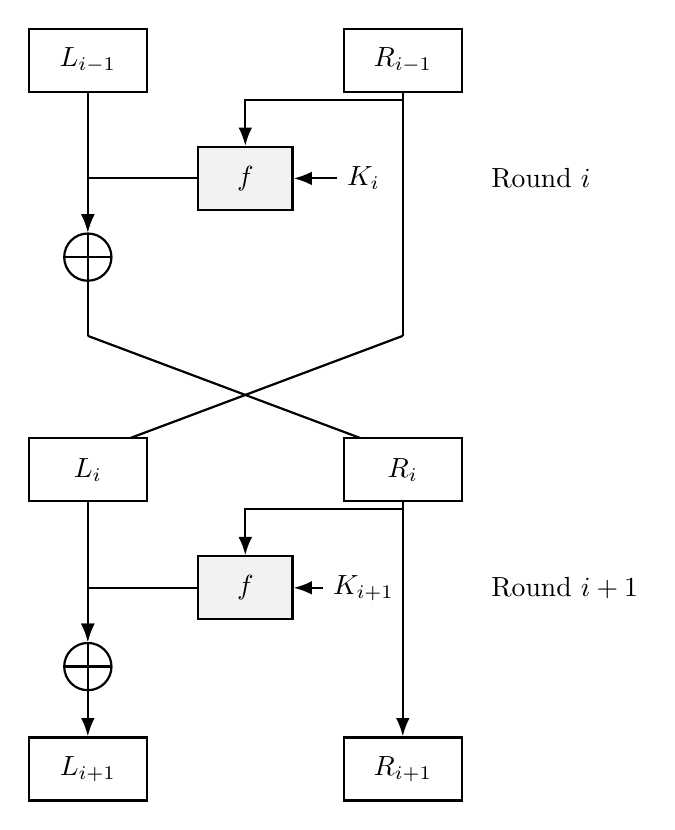
\begin{tikzpicture}[
        % Define styles for consistency
        block/.style={
            rectangle, 
            draw=black, 
            thick, 
            fill=white,
            minimum width=1.5cm, 
            minimum height=0.8cm, 
            align=center,
            font=\bfseries
        },
        func/.style={
            rectangle,
            draw=black,
            thick,
            fill=gray!10,
            minimum width=1.2cm,
            minimum height=0.8cm,
            font=\itshape
        },
        xor/.style={
            circle, 
            draw=black, 
            thick, 
            fill=white,
            minimum size=0.6cm,
            path picture={
                \draw[thick] (path picture bounding box.north) -- (path picture bounding box.south);
                \draw[thick] (path picture bounding box.east) -- (path picture bounding box.west);
            }
        },
        line/.style={
            draw, 
            thick, 
            -Latex
        },
        connector/.style={
            draw, 
            thick
        }
    ]

    % --- ROUND i ---

    % Input Nodes
    \node[block] (Li) at (0,0) {$L_{i-1}$};
    \node[block] (Ri) at (4,0) {$R_{i-1}$};

    % XOR Node on the left side
    \node[xor] (xor1) at (0,-2.5) {};

    % F-Function on the right side logic
    \node[func] (func1) at (2,-1.5) {$f$};
    \node (key1) at (3.5,-1.5) {$K_i$};

    % Connections for Round i
    % Left side vertical flow
    \draw[line] (Li) -- (xor1);
    
    % Right side splits
    \draw[connector] (Ri) -- (4,-2.5); % Main vertical down
    \draw[line] (4,-0.5) -| (func1); % Branch into function
    
    % Key input
    \draw[line] (key1) -- (func1);

    % Function output to XOR
    \draw[line] (func1) -| (xor1);

    % Cross over logic
    % Output of XOR becomes next R
    \coordinate (crossL) at (0,-3.5);
    \coordinate (crossR) at (4,-3.5);
    
    \draw[connector] (xor1) -- (crossL);
    \draw[connector] (4,-2.5) -- (crossR);
    
    % Draw the swap
    \draw[line] (crossL) -- (4,-5); % Left result goes to Right
    \draw[line] (crossR) -- (0,-5); % Right result goes to Left

    % --- ROUND i+1 ---

    % Intermediate Nodes (Ghost nodes for positioning)
    \node[block] (Li1) at (0,-5.2) {$L_{i}$};
    \node[block] (Ri1) at (4,-5.2) {$R_{i}$};

    % XOR Node
    \node[xor] (xor2) at (0,-7.7) {};

    % F-Function
    \node[func] (func2) at (2,-6.7) {$f$};
    \node (key2) at (3.5,-6.7) {$K_{i+1}$};

    % Connections for Round i+1
    \draw[line] (Li1) -- (xor2);
    \draw[connector] (Ri1) -- (4,-7.7);
    \draw[line] (4,-5.7) -| (func2);
    \draw[line] (key2) -- (func2);
    \draw[line] (func2) -| (xor2);

    % Final Outputs
    \node[block] (Li2) at (0,-9) {$L_{i+1}$};
    \node[block] (Ri2) at (4,-9) {$R_{i+1}$};

    % No swap usually in the very last round of DES, 
    % but for generic Feistel rounds, they just continue.
    % We will show them going straight down here to signify end of diagram.
    \draw[line] (xor2) -- (Li2);
    \draw[line] (4,-7.7) -- (Ri2);

    % Annotations
    \node[anchor=west] at (5, -1.5) {Round $i$};
    \node[anchor=west] at (5, -6.7) {Round $i+1$};

    \end{tikzpicture}
    \caption{Two rounds of a Feistel Network structure. Note how $R_{i-1}$ is preserved to become $L_i$, while $L_{i-1}$ is modified by the round function.}
    \label{fig:feistel}
\end{figure}


\subsubsection{Round Key Generation}

\begin{enumerate}
  \item \textbf{Parity Drop (PC-1)}: The process starts with a 64-bit key. However, every 8th bit is a parity bit and is ignored. The remaining 56 bits are shuffled according to "Permuted Choice 1" (PC-1).
  \item \textbf{Splitting}: The 56-bit result is split into two 28-bit halves: $C_0$ and $D_0$.
  \item \textbf{Circular Shifts (Left Rotations)}: In every round, both halves are rotated left by either 1 or 2 bits.
    \begin{itemize}
      \item 1 bit rotation in rounds: 1, 2, 9, 16.
      \item 2 bit rotation in all other rounds
    \end{itemize}
  \item \textbf{Compression (PC-2)}: After shifting, the two halves (56 bits total) are glued back together and passed through "Permuted Choice 2" (PC-2). This selects only 48 specific bits to create the Round Key $(K_i)$.
  \item \textbf{Loop}: The shifted halves $(C_i,D_i)$ are used as the starting point for the next round's shift.
\end{enumerate}

\begin{figure}[H]
    \centering
    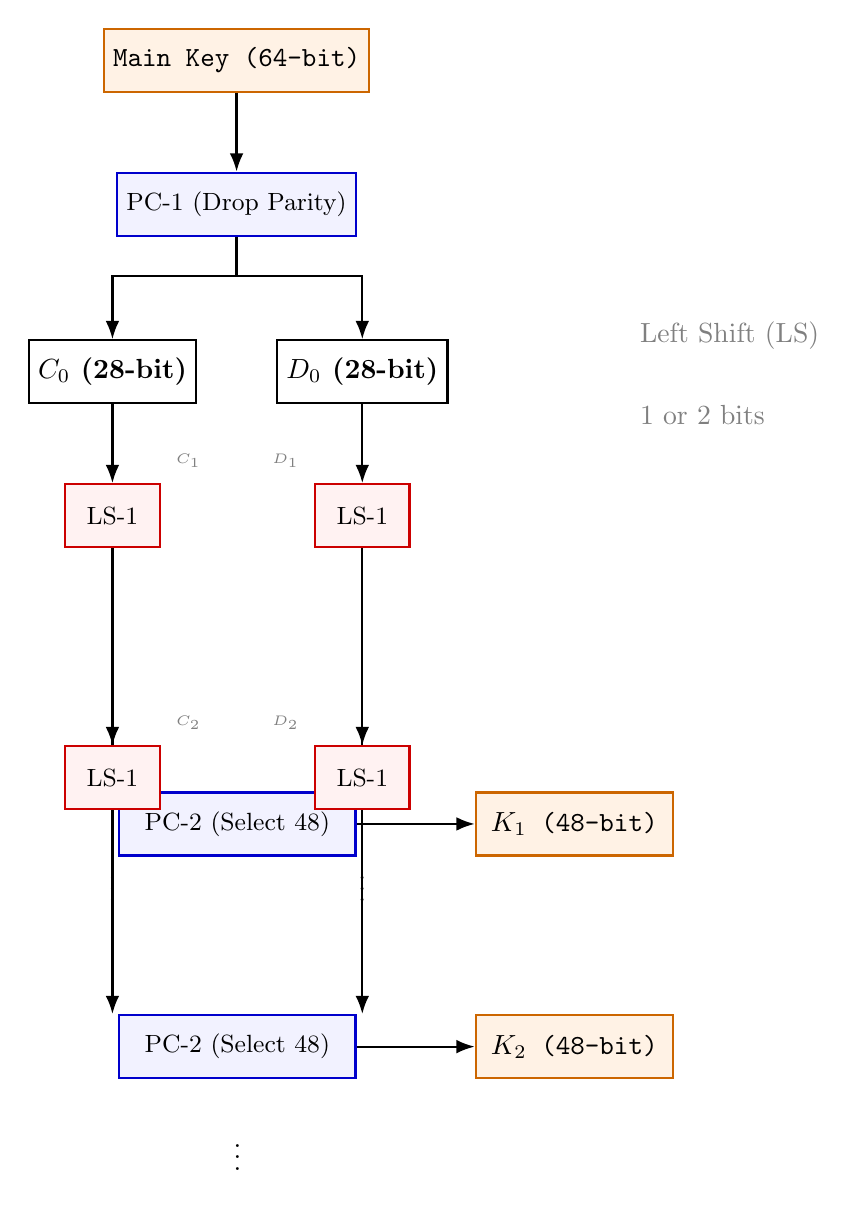
\begin{tikzpicture}[
        node distance=1.5cm,
        % Styles
        block/.style ={rectangle, draw=black, thick, fill=white, minimum width=2cm, minimum height=0.8cm, align=center, font=\bfseries},
        perm/.style  ={rectangle, draw=blue!80!black, thick, fill=blue!5, minimum width=3cm, minimum height=0.8cm, font=\small},
        op/.style    ={rectangle, draw=red!80!black, thick, fill=red!5, minimum width=1.2cm, minimum height=0.8cm, font=\small},
        keybox/.style={rectangle, draw=orange!80!black, thick, fill=orange!10, minimum width=2.5cm, minimum height=0.8cm, font=\ttfamily\bfseries},
        line/.style  ={-Latex, thick},
        connect/.style={thick}
    ]

    % Main Key Input
    \node[keybox] (MainKey) {Main Key (64-bit)};

    % PC-1
    \node[perm, below=1cm of MainKey] (PC1) {PC-1 (Drop Parity)};
    \draw[line] (MainKey) -- (PC1);

    % Split
    \coordinate (split) at ($(PC1.south) + (0,-0.5)$);
    \draw[connect] (PC1.south) -- (split);

    % C0 and D0
    \node[block, below left=0.8cm and 0.5cm of split] (C0) {$C_0$ (28-bit)};
    \node[block, below right=0.8cm and 0.5cm of split] (D0) {$D_0$ (28-bit)};

    \draw[line] (split) -| (C0);
    \draw[line] (split) -| (D0);

    % --- ROUND 1 GENERATION ---
    
    % Shifts
    \node[op, below=1cm of C0] (LS1C) {LS-1};
    \node[op, below=1cm of D0] (LS1D) {LS-1};
    
    \draw[line] (C0) -- (LS1C);
    \draw[line] (D0) -- (LS1D);
    
    % Define C1 D1
    \node[above right=0.1cm of LS1C, font=\tiny, color=gray] {$C_1$};
    \node[above left=0.1cm of LS1D, font=\tiny, color=gray] {$D_1$};

    % PC-2 (Compression)
    % Merge lines from shift output to PC-2
    \node[perm, below=2cm of split] (PC2_1) at ($(LS1C)!0.5!(LS1D) + (0,-1.5)$) {PC-2 (Select 48)};
    
    % Draw connections to PC-2
    \draw[line] (LS1C.south) -- ++(0,-0.3) -- (LS1C.south |- PC2_1.north); 
    \draw[line] (LS1D.south) -- ++(0,-0.3) -- (LS1D.south |- PC2_1.north);

    % Output Key 1
    \node[keybox, right=1.5cm of PC2_1] (K1) {$K_1$ (48-bit)};
    \draw[line] (PC2_1) -- (K1);


    % --- ROUND 2 GENERATION ---

    % Shifts (LS-2 usually, depends on schedule)
    \node[op, below=2.5cm of LS1C] (LS2C) {LS-1};
    \node[op, below=2.5cm of LS1D] (LS2D) {LS-1};

    % Connect previous shift output to next shift input
    % We draw a line bypassing PC-2
    \draw[line] (LS1C.south) -- ++(0,-0.5) -- (LS2C.north);
    \draw[line] (LS1D.south) -- ++(0,-0.5) -- (LS2D.north);

    % Define C2 D2
    \node[above right=0.1cm of LS2C, font=\tiny, color=gray] {$C_2$};
    \node[above left=0.1cm of LS2D, font=\tiny, color=gray] {$D_2$};

    % PC-2 Round 2
    \node[perm, below=2cm of PC2_1] (PC2_2) {PC-2 (Select 48)};
    
    \draw[line] (LS2C.south) -- ++(0,-0.3) -- (LS2C.south |- PC2_2.north);
    \draw[line] (LS2D.south) -- ++(0,-0.3) -- (LS2D.south |- PC2_2.north);

    % Output Key 2
    \node[keybox, right=1.5cm of PC2_2] (K2) {$K_2$ (48-bit)};
    \draw[line] (PC2_2) -- (K2);

    % ... Continuation
    \node[below=0.5cm of LS2C] {$\vdots$};
    \node[below=0.5cm of LS2D] {$\vdots$};
    \node[below=0.5cm of PC2_2] {$\vdots$};

    % Annotations
    \node[anchor=west, text=gray] at (5, -3.5) {Left Shift (LS)};
    \node[anchor=west, text=gray] at (5, -4.5) {1 or 2 bits};

    \end{tikzpicture}
    \caption{The DES Key Schedule. The 56-bit key state ($C, D$) is rotated left every round. The PC-2 permutation compresses the state to produce the 48-bit round key.}
    \label{fig:key_schedule}
\end{figure}


\begin{figure}[H]
    \centering
    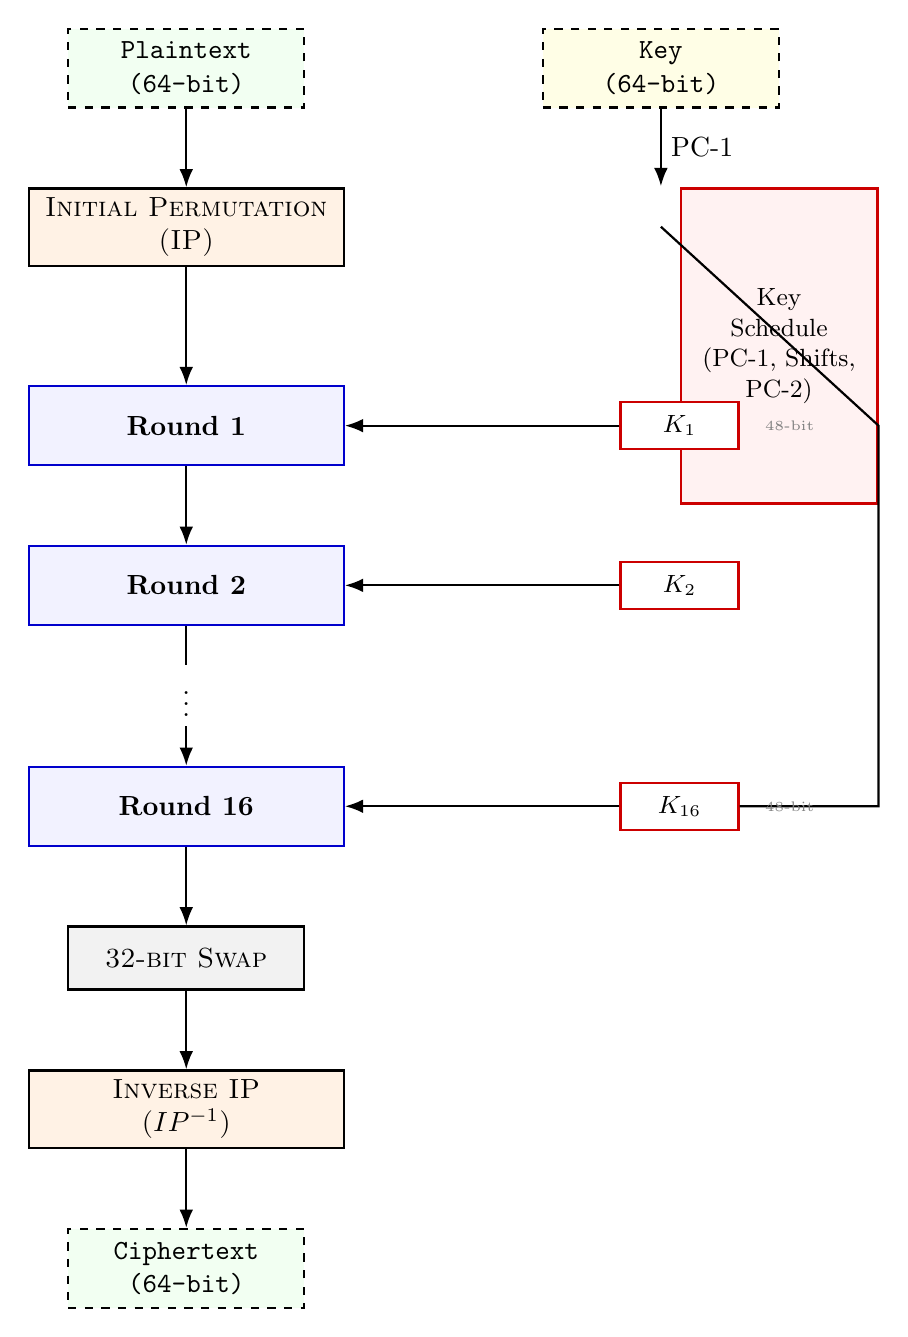
\begin{tikzpicture}[
        node distance=1.5cm,
        % Styles
        io/.style    ={rectangle, draw=black, dashed, thick, fill=green!5, minimum width=3cm, minimum height=1cm, align=center, font=\ttfamily},
        % Added align=center to allow line breaks (\\) inside the node
        perm/.style  ={rectangle, draw=black, thick, fill=orange!10, minimum width=4cm, minimum height=0.8cm, align=center, font=\scshape},
        round/.style ={rectangle, draw=blue!80!black, thick, fill=blue!5, minimum width=4cm, minimum height=1cm, align=center, font=\bfseries},
        keyproc/.style={rectangle, draw=red!80!black, thick, fill=red!5, minimum width=2.5cm, minimum height=4cm, align=center, font=\small},
        keynode/.style={rectangle, draw=red!80!black, thick, fill=white, minimum width=1.5cm, minimum height=0.6cm, font=\ttfamily\small},
        line/.style  ={-Latex, thick},
        connect/.style={thick}
    ]

    % --- MAIN DATA PATH (Left Side) ---

    % Plaintext
    \node[io] (Plaintext) {Plaintext\\(64-bit)};

    % Initial Permutation
    \node[perm, below=1cm of Plaintext] (IP) {Initial Permutation\\(IP)};
    \draw[line] (Plaintext) -- (IP);

    % Round 1
    \node[round, below=1.5cm of IP] (R1) {Round 1};
    \draw[line] (IP) -- (R1);

    % Round 2
    \node[round, below=1cm of R1] (R2) {Round 2};
    \draw[line] (R1) -- (R2);

    % Dots
    \node[below=0.5cm of R2] (dots) {$\vdots$};
    \draw[connect] (R2) -- (dots);

    % Round 16
    \node[round, below=0.5cm of dots] (R16) {Round 16};
    \draw[line] (dots) -- (R16);

    % 32-bit Swap
    \node[perm, below=1cm of R16, fill=gray!10, minimum width=3cm] (Swap) {32-bit Swap};
    \draw[line] (R16) -- (Swap);

    % Inverse IP
    \node[perm, below=1cm of Swap] (InvIP) {Inverse IP\\($IP^{-1}$)};
    \draw[line] (Swap) -- (InvIP);

    % Ciphertext
    \node[io, below=1cm of InvIP] (Ciphertext) {Ciphertext\\(64-bit)};
    \draw[line] (InvIP) -- (Ciphertext);


    % --- KEY SCHEDULE SIDE (Right Side) ---

    % Main Key
    \node[io, right=3cm of Plaintext, fill=yellow!10] (MainKey) {Key\\(64-bit)};

    % Key Schedule Logic Block (Abstracted)
    % We draw a visual container for the key generation
    \node[keyproc, right=1.5cm of R1, anchor=north] (KeySched) at ($(MainKey.south) + (0,-1)$) {Key\\Schedule\\(PC-1, Shifts,\\PC-2)};
    
    % Resize KeySched to span the rounds using the fit library
    \node[keyproc, fit=(KeySched) (R16 |- KeySched.south), inner sep=0pt, draw=none, fill=none] {}; 

    % Draw Key Flow
    \draw[line] (MainKey) -- ++(0,-1.5) node[midway, right] {PC-1};
    
    % Subkeys
    \node[keynode] (K1) at (KeySched.west |- R1) {$K_1$};
    \node[keynode] (K2) at (KeySched.west |- R2) {$K_2$};
    \node[keynode] (K16) at (KeySched.west |- R16) {$K_{16}$};

    % Connect Schedule to Subkeys
    \draw[connect] (MainKey.south) ++(0,-1.5) -- (K1.east -| KeySched.east) -- (KeySched.east |- K16.east) -- (K16.east);
    
    % Connect Subkeys to Rounds
    \draw[line] (K1) -- (R1);
    \draw[line] (K2) -- (R2);
    \draw[line] (K16) -- (R16);

    % Annotations
    \node[right=0.2cm of K1, font=\tiny, text=gray] {48-bit};
    \node[right=0.2cm of K16, font=\tiny, text=gray] {48-bit};

    \end{tikzpicture}
    \caption{Overview of the Full DES Algorithm. The 64-bit Plaintext undergoes an Initial Permutation, 16 Rounds of processing (each using a unique 48-bit subkey derived from the main 64-bit Key), a final swap, and an Inverse Permutation.}
    \label{fig:full_des}
\end{figure}


\section{Advanced Encryption Standard (AES)}

\begin{itemize}
  \item Block size: 128 bits
  \item Key Sizes: 128, 192, 256 bits
  \item Number of processing rounds depends on the key length:
    \begin{itemize}
      \item 128: 10 rounds
      \item 192: 12 rounds
      \item 256: 14 rounds
    \end{itemize}
\end{itemize}

AES treats data blocks as 4x4 matrix of bytes $\rightarrow$ \textbf{State}.


\subsection{1. SubBytes (Substitution)}


This is the only non-linear transformation in the cipher. Each byte in the state is independently replaced by another byte from a fixed 8-bit Lookup Table (S-Box).


\begin{figure}[H]
    \centering
    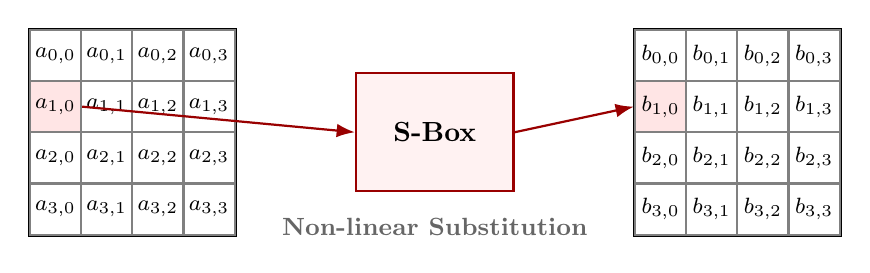
\begin{tikzpicture}
        % Input State
        \matrix[state] (In) {
            $a_{0,0}$ & $a_{0,1}$ & $a_{0,2}$ & $a_{0,3}$ \\
            |[fill=red!10]| $a_{1,0}$ & $a_{1,1}$ & $a_{1,2}$ & $a_{1,3}$ \\
            $a_{2,0}$ & $a_{2,1}$ & $a_{2,2}$ & $a_{2,3}$ \\
            $a_{3,0}$ & $a_{3,1}$ & $a_{3,2}$ & $a_{3,3}$ \\
        };
        
        % S-Box Box
        \node[rectangle, draw=red!60!black, fill=red!5, thick, minimum width=2cm, minimum height=1.5cm, right=1.5cm of In] (SBox) {\textbf{S-Box}};
        
        % Output State
        \matrix[state, right=1.5cm of SBox] (Out) {
            $b_{0,0}$ & $b_{0,1}$ & $b_{0,2}$ & $b_{0,3}$ \\
            |[fill=red!10]| $b_{1,0}$ & $b_{1,1}$ & $b_{1,2}$ & $b_{1,3}$ \\
            $b_{2,0}$ & $b_{2,1}$ & $b_{2,2}$ & $b_{2,3}$ \\
            $b_{3,0}$ & $b_{3,1}$ & $b_{3,2}$ & $b_{3,3}$ \\
        };
        
        % Arrows
        \draw[arrow, red!60!black] (In-2-1.east) -- (SBox.west);
        \draw[arrow, red!60!black] (SBox.east) -- (Out-2-1.west);
        
        \node[label, below=0.2cm of SBox] {Non-linear Substitution};
    \end{tikzpicture}
    \caption{SubBytes: Each byte is replaced individually.}
\end{figure}

\subsection{2. ShiftRows (Permutation)}


This step provides diffusion among the columns. The rows of the state are shifted cyclically to the left.
\begin{itemize}
    \item \textbf{Row 0:} Not shifted.
    \item \textbf{Row 1:} Shifted left by 1 byte.
    \item \textbf{Row 2:} Shifted left by 2 bytes.
    \item \textbf{Row 3:} Shifted left by 3 bytes.
\end{itemize}

\begin{figure}[H]
    \centering
    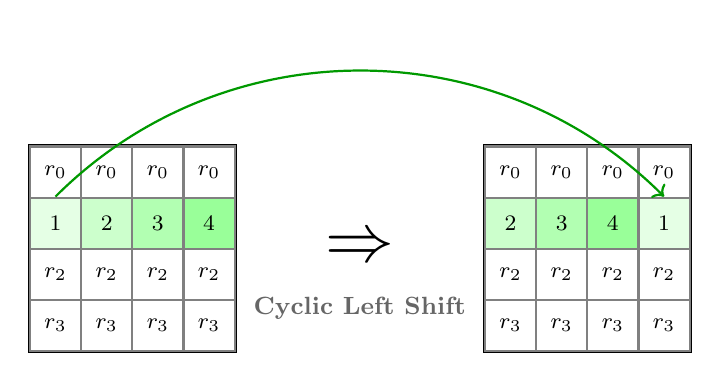
\begin{tikzpicture}
        % Input State
        \matrix[state] (In) {
            $r_0$ & $r_0$ & $r_0$ & $r_0$ \\
            |[fill=green!10]| $1$ & |[fill=green!20]| $2$ & |[fill=green!30]| $3$ & |[fill=green!40]| $4$ \\
            $r_2$ & $r_2$ & $r_2$ & $r_2$ \\
            $r_3$ & $r_3$ & $r_3$ & $r_3$ \\
        };
        
        \node[right=1cm of In] (Arrow) {\Huge $\Rightarrow$};
        
        % Output State
        \matrix[state, right=1cm of Arrow] (Out) {
            $r_0$ & $r_0$ & $r_0$ & $r_0$ \\
            |[fill=green!20]| $2$ & |[fill=green!30]| $3$ & |[fill=green!40]| $4$ & |[fill=green!10]| $1$ \\
            $r_2$ & $r_2$ & $r_2$ & $r_2$ \\
            $r_3$ & $r_3$ & $r_3$ & $r_3$ \\
        };
        
        % Visualizing the shift for Row 1
        \draw[->, thick, green!60!black] (In-2-1.north) to[bend left=45] (Out-2-4.north);
        \node[label, below=0.2cm of Arrow] {Cyclic Left Shift};
    \end{tikzpicture}
    \caption{ShiftRows: Row 1 is shifted left by 1. Byte '1' wraps around to the end.}
\end{figure}

\subsection{3. MixColumns (Diffusion)}


This transformation operates on the State column-by-column, treating each column as a four-term polynomial. The columns are multiplied by a fixed matrix over $GF(2^8)$. This step is omitted in the final round.

\begin{figure}[H]
    \centering
    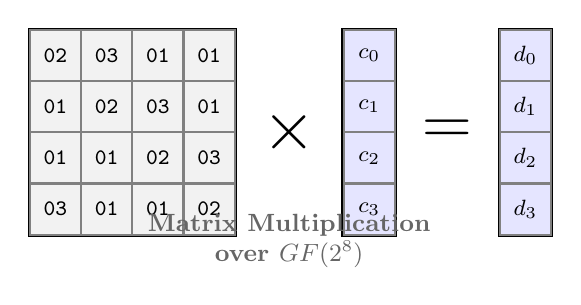
\begin{tikzpicture}
        % Matrix M
        \matrix[state, nodes={fill=gray!10}] (M) {
            02 & 03 & 01 & 01 \\
            01 & 02 & 03 & 01 \\
            01 & 01 & 02 & 03 \\
            03 & 01 & 01 & 02 \\
        };
        
        \node[right=0.2cm of M] (Times) {\Huge $\times$};
        
        % Column Input
        \matrix[state, right=0.2cm of Times, nodes={fill=blue!10}] (ColIn) {
            $c_0$ \\ $c_1$ \\ $c_2$ \\ $c_3$ \\
        };
        
        \node[right=0.2cm of ColIn] (Equals) {\Huge $=$};
        
        % Column Output
        \matrix[state, right=0.2cm of Equals, nodes={fill=blue!10}] (ColOut) {
            $d_0$ \\ $d_1$ \\ $d_2$ \\ $d_3$ \\
        };
        
        \node[label, below=0.5cm of Times] {Matrix Multiplication\\over $GF(2^8)$};
    \end{tikzpicture}
    \caption{MixColumns: Each column is transformed linearly.}
\end{figure}

\subsection{4. AddRoundKey (Key Mixing)}


A Round Key is combined with the State by a simple bitwise XOR operation. This is the encryption step that injects the secret key into the state.

\begin{figure}[H]
    \centering
    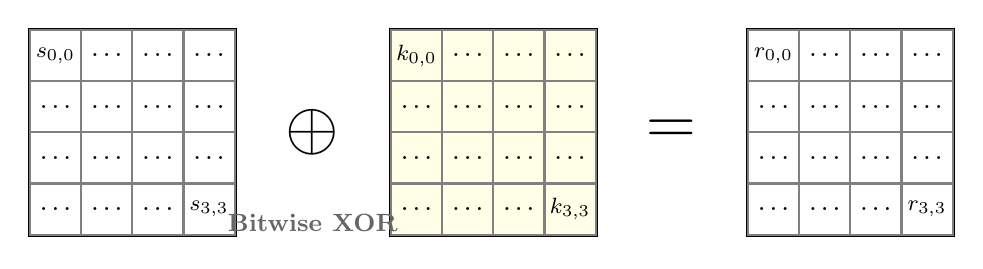
\begin{tikzpicture}
        % State
        \matrix[state] (State) {
            $s_{0,0}$ & \dots & \dots & \dots \\
            \dots & \dots & \dots & \dots \\
            \dots & \dots & \dots & \dots \\
            \dots & \dots & \dots & $s_{3,3}$ \\
        };
        
        \node[right=0.5cm of State] (XOR) {\Huge $\oplus$};
        
        % Key
        \matrix[state, right=0.5cm of XOR, nodes={fill=yellow!10}] (Key) {
            $k_{0,0}$ & \dots & \dots & \dots \\
            \dots & \dots & \dots & \dots \\
            \dots & \dots & \dots & \dots \\
            \dots & \dots & \dots & $k_{3,3}$ \\
        };
        
         \node[right=0.5cm of Key] (Equals) {\Huge $=$};
         
         % Result
        \matrix[state, right=0.5cm of Equals] (Result) {
            $r_{0,0}$ & \dots & \dots & \dots \\
            \dots & \dots & \dots & \dots \\
            \dots & \dots & \dots & \dots \\
            \dots & \dots & \dots & $r_{3,3}$ \\
        };

        \node[label, below=0.5cm of XOR] {Bitwise XOR};
    \end{tikzpicture}
    \caption{AddRoundKey: The internal State is XORed with the Round Key.}
\end{figure}




AES requires a separate 128-bit key for each round (plus one initial key). This means for AES-128, we need 11 keys ($4 \times 11 = 44$ words).

\subsection{Expansion Algorithm}
The expansion uses a recursive logic. Let $W_i$ be the $i$-th 32-bit word of the key schedule:
\begin{enumerate}
    \item If $i < 4$ (First 4 words): $W_i = \text{InputKeyWord}_i$.
    \item If $i \geq 4$:
    \begin{itemize}
        \item If $i$ is a multiple of 4: $W_i = W_{i-4} \oplus g(W_{i-1})$.
        \item Otherwise: $W_i = W_{i-4} \oplus W_{i-1}$.
    \end{itemize}
\end{enumerate}

\subsection{The $g()$ Function}
For every 4th word, a complex transformation $g()$ is applied to ensure non-linearity and break symmetries:
\begin{enumerate}
    \item \textbf{RotWord:} A 1-byte left circular shift. $[b_0, b_1, b_2, b_3] \to [b_1, b_2, b_3, b_0]$.
    \item \textbf{SubWord:} Apply the S-Box to each of the 4 bytes.
    \item \textbf{Round Constant (Rcon):} XOR the first byte with $Rcon_j$ (where $j$ is the round number).
\end{enumerate}

\begin{table}[H]
    \centering
    \begin{tabular}{ccccccccccc}
        \toprule
        \textbf{Round ($j$)} & 1 & 2 & 3 & 4 & 5 & 6 & 7 & 8 & 9 & 10 \\
        \midrule
        \textbf{Rcon$_j$ (hex)} & 01 & 02 & 04 & 08 & 10 & 20 & 40 & 80 & 1B & 36 \\
        \bottomrule
    \end{tabular}
    \caption{Rcon values for each round (only affects the first byte of the word).}
\end{table}

\begin{figure}[H]
    \centering
    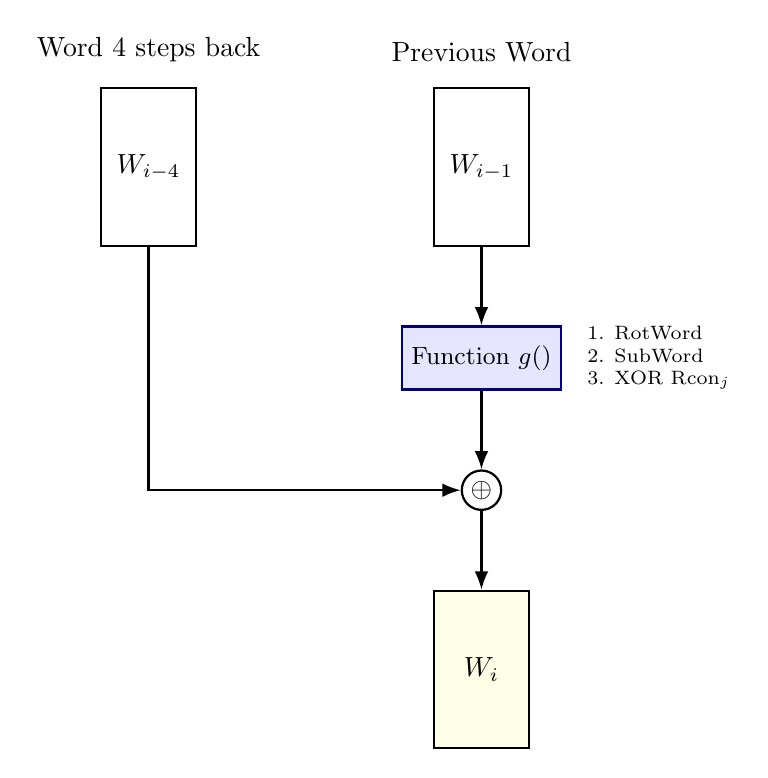
\begin{tikzpicture}[
        word/.style={rectangle, draw=black, thick, minimum width=1.2cm, minimum height=2cm, align=center, fill=white},
        op/.style={circle, draw=black, thick, inner sep=0pt, minimum size=0.5cm},
        func/.style={rectangle, draw=blue!50!black, thick, fill=blue!10, minimum width=2cm, minimum height=0.8cm, font=\small}
    ]
    
    % Previous Words
    \node[word] (Wi-1) {$W_{i-1}$};
    \node[word, left=3cm of Wi-1] (Wi-4) {$W_{i-4}$};
    
    % Function g
    \node[func, below=1cm of Wi-1] (G) {Function $g()$};
    \node[right=0.2cm of G, font=\scriptsize, align=left] {1. RotWord\\2. SubWord\\3. XOR Rcon$_j$};
    
    % XOR Operation
    \node[op, below=1cm of G] (XOR) {$\oplus$};
    
    % Result
    \node[word, below=1cm of XOR, fill=yellow!10] (Wi) {$W_i$};
    
    % Connections
    \draw[-Latex, thick] (Wi-1) -- (G);
    \draw[-Latex, thick] (G) -- (XOR);
    \draw[-Latex, thick] (Wi-4) |- (XOR);
    \draw[-Latex, thick] (XOR) -- (Wi);
    
    \node[above=0.2cm of Wi-4] {Word 4 steps back};
    \node[above=0.2cm of Wi-1] {Previous Word};

    \end{tikzpicture}
    \caption{Key Expansion Logic (for indices $i$ multiple of 4).}
\end{figure}

\subsection{Complete Process}

\begin{figure}[H]
    \centering
    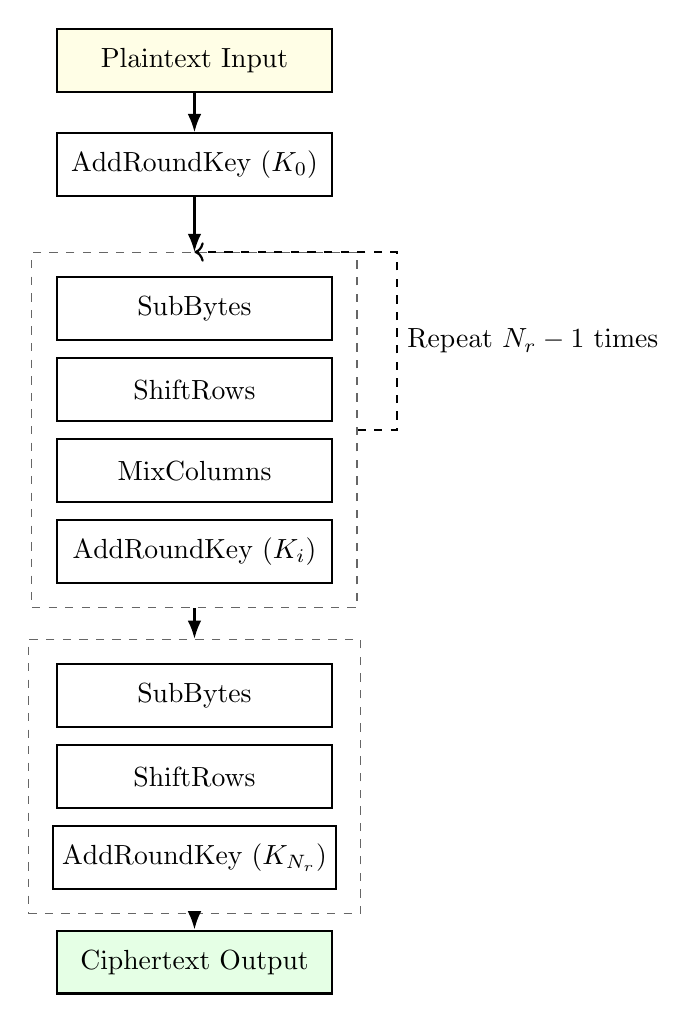
\begin{tikzpicture}[
        process/.style={rectangle, draw=black, thick, fill=white, align=center, minimum width=3.5cm, minimum height=0.8cm},
        group/.style={rectangle, draw=gray, dashed, inner sep=0.3cm},
        arrow/.style={-Latex, thick}
    ]
        % Nodes
        \node[process, fill=yellow!10] (Start) {Plaintext Input};
        \node[process, below=0.5cm of Start] (Init) {AddRoundKey ($K_0$)};
        
        % Main Loop
        \node[process, below=1cm of Init] (Sub) {SubBytes};
        \node[process, below=0.2cm of Sub] (Shift) {ShiftRows};
        \node[process, below=0.2cm of Shift] (Mix) {MixColumns};
        \node[process, below=0.2cm of Mix] (Add) {AddRoundKey ($K_i$)};
        
        \node[group, fit=(Sub) (Add), label=left:\rotatebox{90}{\textbf{Main Rounds}}] (MainGroup) {};
        
        % Final Round
        \node[process, below=1cm of Add] (FSub) {SubBytes};
        \node[process, below=0.2cm of FSub] (FShift) {ShiftRows};
        \node[process, below=0.2cm of FShift] (FAdd) {AddRoundKey ($K_{N_r}$)};
        
        \node[group, fit=(FSub) (FAdd), label=left:\rotatebox{90}{\textbf{Final Round}}] (FinalGroup) {};
        
        \node[process, below=0.5cm of FAdd, fill=green!10] (End) {Ciphertext Output};

        % Edges
        \draw[arrow] (Start) -- (Init);
        \draw[arrow] (Init) -- (MainGroup);
        \draw[arrow] (MainGroup) -- (FinalGroup);
        \draw[arrow] (FinalGroup) -- (End);
        
        % Loop annotation
        \draw[->, thick, dashed] (MainGroup.east) -- ++(0.5,0) |- (MainGroup.north) node[pos=0.25, right] {Repeat $N_r-1$ times};

    \end{tikzpicture}
    \caption{AES Execution Flow.}
\end{figure}

\section{AES modes}


\subsection{ECB (Electronic Codebook)}
The simplest mode. Each block is encrypted independently.
\begin{itemize}
    \item \textbf{Weakness:} Identical plaintext blocks produce identical ciphertext blocks. This preserves patterns (e.g., the famous "Penguin" image remains visible).
    \item \textbf{Use Case:} Almost never recommended.
\end{itemize}

\subsection{CBC (Cipher Block Chaining)}
Each block of plaintext is XORed with the previous ciphertext block before being encrypted. This randomizes the output.
\begin{itemize}
    \item \textbf{IV (Initialization Vector):} Required for the first block to ensure uniqueness.
    \item \textbf{Sequential:} Cannot parallelize encryption (must wait for previous block).
\end{itemize}

\begin{figure}[H]
    \centering
    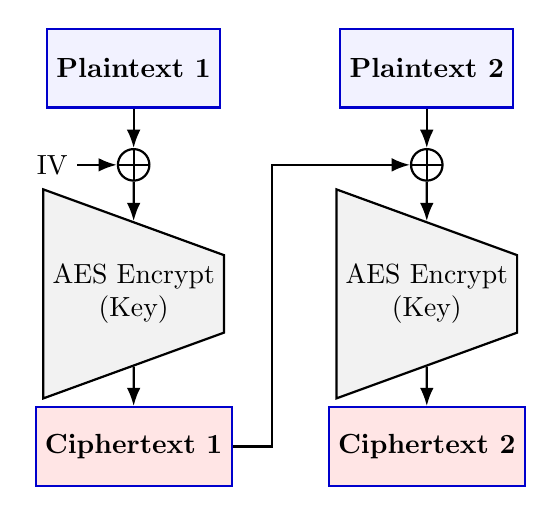
\begin{tikzpicture}[node distance=1.5cm]
        % Block 1
        \node[block] (P1) {Plaintext 1};
        \node[xor, below=0.5cm of P1] (XOR1) {};
        \node[left=0.5cm of XOR1] (IV) {IV};
        \node[enc, below=0.5cm of XOR1] (E1) {AES Encrypt\\(Key)};
        \node[block, below=0.5cm of E1, fill=red!10] (C1) {Ciphertext 1};
        
        % Block 2
        \node[block, right=1.5cm of P1] (P2) {Plaintext 2};
        \node[xor, below=0.5cm of P2] (XOR2) {};
        \node[enc, below=0.5cm of XOR2] (E2) {AES Encrypt\\(Key)};
        \node[block, below=0.5cm of E2, fill=red!10] (C2) {Ciphertext 2};

        % Connections 1
        \draw[arrow] (P1) -- (XOR1);
        \draw[arrow] (IV) -- (XOR1);
        \draw[arrow] (XOR1) -- (E1);
        \draw[arrow] (E1) -- (C1);

        % Connections 2
        \draw[arrow] (P2) -- (XOR2);
        \draw[arrow] (C1.east) -- ++(0.5,0) |- (XOR2.west);
        \draw[arrow] (XOR2) -- (E2);
        \draw[arrow] (E2) -- (C2);
    \end{tikzpicture}
    \caption{Cipher Block Chaining (CBC) Mode.}
\end{figure}

\subsection{CTR (Counter Mode)}
Turns the block cipher into a \textit{Stream Cipher}. It generates a keystream by encrypting a counter, which is then XORed with the plaintext.
\begin{itemize}
    \item \textbf{Parallelizable:} Blocks can be encrypted simultaneously.
    \item \textbf{No Padding:} The ciphertext is exactly the same length as the plaintext.
\end{itemize}

\begin{figure}[H]
    \centering
    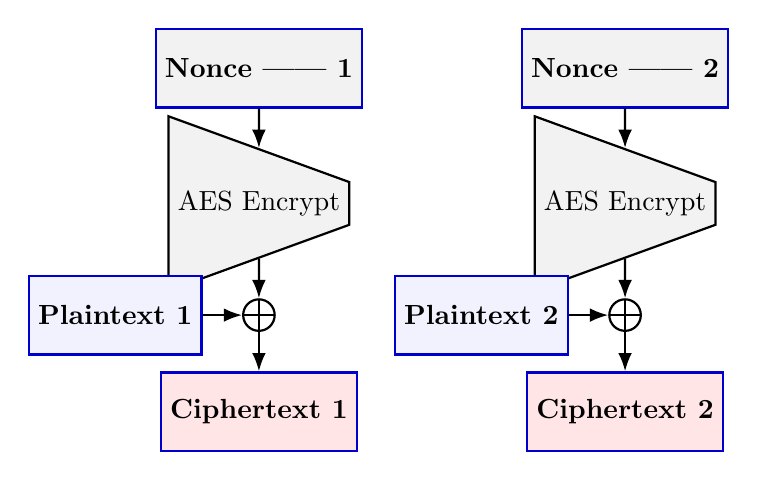
\begin{tikzpicture}[node distance=1.5cm]
        % Block 1
        \node[block, fill=gray!10] (Ctr1) {Nonce || 1};
        \node[enc, below=0.5cm of Ctr1] (E1) {AES Encrypt};
        \node[xor, below=0.5cm of E1] (XOR1) {};
        \node[block, left=0.5cm of XOR1] (P1) {Plaintext 1};
        \node[block, below=0.5cm of XOR1, fill=red!10] (C1) {Ciphertext 1};
        
        % Block 2
        \node[block, fill=gray!10, right=2cm of Ctr1] (Ctr2) {Nonce || 2};
        \node[enc, below=0.5cm of Ctr2] (E2) {AES Encrypt};
        \node[xor, below=0.5cm of E2] (XOR2) {};
        \node[block, left=0.5cm of XOR2] (P2) {Plaintext 2};
        \node[block, below=0.5cm of XOR2, fill=red!10] (C2) {Ciphertext 2};

        % Connections
        \draw[arrow] (Ctr1) -- (E1);
        \draw[arrow] (E1) -- (XOR1);
        \draw[arrow] (P1) -- (XOR1);
        \draw[arrow] (XOR1) -- (C1);

        \draw[arrow] (Ctr2) -- (E2);
        \draw[arrow] (E2) -- (XOR2);
        \draw[arrow] (P2) -- (XOR2);
        \draw[arrow] (XOR2) -- (C2);
    \end{tikzpicture}
    \caption{Counter (CTR) Mode.}
\end{figure}

\subsection{GCM (Galois/Counter Mode)}
Currently the most popular mode (used in HTTPS/TLS). It combines \textbf{CTR mode} for encryption with a Galois Field multiplication for \textbf{Authentication} (integrity).
\begin{itemize}
    \item Provides both confidentiality and authenticity.
    \item Highly efficient (parallelizable).
\end{itemize}


\section{Block ciphers vs Stream ciphers}

\subsection{Block Ciphers}
A block cipher breaks the plaintext into fixed-size chunks called \textbf{blocks} (e.g., 64 bits for DES, 128 bits for AES). It then encrypts each block independently (or chained together) using the secret key.

\subsubsection*{Characteristics}
\begin{itemize}
    \item \textbf{Fixed Input Size:} Data must be padded if it doesn't fit the block size perfectly.
    \item \textbf{Complex Internals:} Uses "Confusion and Diffusion" (Substitution-Permutation Networks or Feistel Networks).
    \item \textbf{Modes of Operation:} Requires a mode (like CBC, GCM) to securely encrypt messages longer than one block.
\end{itemize}

\begin{figure}[H]
    \centering
    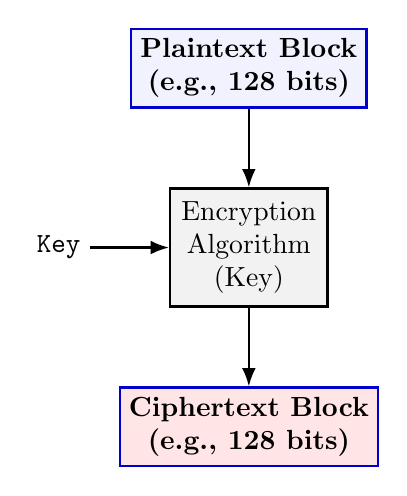
\begin{tikzpicture}[
        block/.style={rectangle, draw=blue!80!black, thick, fill=blue!5, minimum width=2.5cm, minimum height=1cm, align=center, font=\bfseries},
        enc/.style={rectangle, draw=black, thick, fill=gray!10, minimum width=2cm, minimum height=1.5cm, align=center},
        arrow/.style={-Latex, thick}
    ]
        % Nodes
        \node[block] (P) {Plaintext Block\\(e.g., 128 bits)};
        \node[enc, below=1cm of P] (E) {Encryption\\Algorithm\\(Key)};
        \node[block, below=1cm of E, fill=red!10] (C) {Ciphertext Block\\(e.g., 128 bits)};
        
        % Key
        \node[left=1cm of E, font=\ttfamily] (K) {Key};
        
        % Edges
        \draw[arrow] (P) -- (E);
        \draw[arrow] (K) -- (E);
        \draw[arrow] (E) -- (C);
        
    \end{tikzpicture}
    \caption{Block Cipher Concept: Transforming a whole chunk at once.}
\end{figure}

\subsection{Stream Ciphers}
A stream cipher processes data **one bit (or byte) at a time**. It functions by generating a pseudorandom stream of bits (called the \textit{Keystream}) from the secret key and XORing it with the plaintext.

\subsubsection*{Characteristics}
\begin{itemize}
    \item \textbf{Continuous Flow:} No padding required; ciphertext is the same length as plaintext.
    \item \textbf{Speed:} Generally faster and simpler in hardware than block ciphers.
    \item \textbf{Simplicity:} Often just XOR operations combined with a state update function.
    \item \textbf{Error Propagation:} A bit-flip error in ciphertext affects only that specific bit in plaintext (unlike block ciphers where it ruins the whole block).
\end{itemize}

\begin{figure}[H]
    \centering
    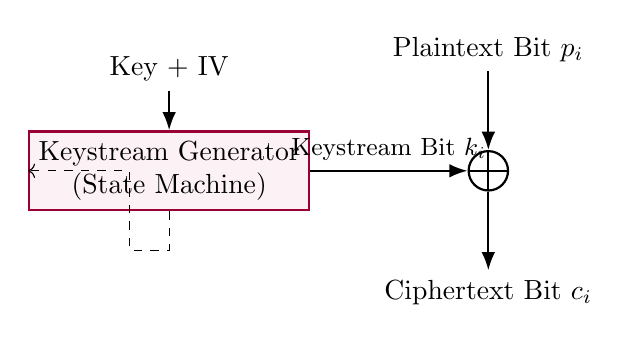
\begin{tikzpicture}[
        bit/.style={circle, draw=black, minimum size=0.6cm, font=\ttfamily},
        gen/.style={rectangle, draw=purple!80!black, thick, fill=purple!5, minimum width=3cm, minimum height=1cm, align=center},
        xor/.style={circle, draw=black, thick, inner sep=0pt, minimum size=0.5cm, path picture={\draw[thick] (path picture bounding box.north) -- (path picture bounding box.south) (path picture bounding box.west) -- (path picture bounding box.east);}},
        arrow/.style={-Latex, thick}
    ]
        % Generator
        \node[gen] (G) {Keystream Generator\\(State Machine)};
        \node[above=0.5cm of G] (Key) {Key + IV};
        \draw[arrow] (Key) -- (G);

        % Flow
        \node[xor, right=2cm of G] (XOR) {};
        \node[above=1cm of XOR] (P) {Plaintext Bit $p_i$};
        \node[below=1cm of XOR] (C) {Ciphertext Bit $c_i$};
        
        % Edges
        \draw[arrow] (G) -- node[midway, above, font=\small] {Keystream Bit $k_i$} (XOR);
        \draw[arrow] (P) -- (XOR);
        \draw[arrow] (XOR) -- (C);
        
        % Loop hint
        \draw[->, dashed] (G.south) |- ++(-0.5, -0.5) |- (G.west);

    \end{tikzpicture}
    \caption{Stream Cipher Concept: XORing data with a running keystream.}
\end{figure}

\subsection{Comparison Summary}

\begin{table}[H]
    \centering
    \renewcommand{\arraystretch}{1.5}
    \begin{tabular}{@{} p{3.5cm} p{5.5cm} p{5.5cm} @{}}
        \toprule
        \textbf{Feature} & \textbf{Block Cipher} & \textbf{Stream Cipher} \\
        \midrule
        \textbf{Unit of Processing} & Large Blocks (64/128 bits) & Bits or Bytes (1 at a time) \\
        \textbf{Examples} & AES, DES, 3DES, Blowfish & RC4, ChaCha20, Salsa20 \\
        \textbf{Complexity} & High (Complex transformations) & Low (XOR + State update) \\
        \textbf{Speed} & Slower (unless hardware accelerated) & Very Fast \\
        \textbf{Error Propagation} & One bit error corrupts whole block & One bit error affects only one bit \\
        \textbf{Padding} & Often required & Not required \\
        \textbf{Primary Use} & File storage, SSL/TLS, Database encryption & Real-time communications, Mobile, IoT \\
        \bottomrule
    \end{tabular}
    \caption{Key differences between Block and Stream ciphers.}
\end{table}

\section{Assimetric Encryption}

An assymetric encryption scheme is consists of three, polinomial time functions $(Gen, Enc, Dec)$ so:

\begin{itemize}
  \item \textbf{$Gen$ Key Generation Algorithm}: $Gen$ takes $1^n$ security parameter as input and outputs the keypair $(pk, sk)$, whereas the $pk$ is the public key and $sk$ is the secret key.
  We assume that $sk$ and $pk$ has the size of at least $n$, and $n$ can be defined from $(pk, sk)$. $(pk, sk) \leftarrow Gen(1^n)$
  \item \textbf{$Enc$ Encryption Algorithm}: $Enc$ takes $pk$ and $m \in \mathcal{M}$ as inputs, and outputs $c \in \mathcal{C}$ ciphertext. $c \leftarrow Enc_{pk}(m)$
  \item \textbf{$Dec$ Decryption Algorithm}: $Dec$ takes $sk$ and $c \in \mathcal{C}$ as inputs, and outputs the original message $m$ or returns error symbol $\perp$. $m \leftarrow Dec_{sk}(c)$
\end{itemize}

We require that $Dec_{sk}(Enc_{pk}(m)) = m$

\subsection{The RSA Problem}
The security of the RSA cryptosystem is based on the difficulty of taking $e$-th roots modulo a composite number $n$.

\subsubsection*{Definition}
Given:
\begin{itemize}
    \item A large composite integer $n = p \cdot q$ (where $p$ and $q$ are unknown large primes).
    \item A public exponent $e$ such that $\gcd(e, \phi(n)) = 1$.
    \item A ciphertext $c \in \mathbb{Z}_n^*$.
\end{itemize}
\textbf{The Problem}: Find the integer $m$ such that:
\[ m^e \equiv c \pmod n \]

\subsubsection*{Relation to Factoring}
The RSA assumption is closely related to the \textbf{Integer Factorization Problem}: Given $n$, find $p$ and $q$.
\begin{itemize}
    \item If an attacker can factor $n$, they can calculate $\phi(n) = (p-1)(q-1)$, compute the private key $d \equiv e^{-1} \pmod{\phi(n)}$, and trivially solve the RSA problem.
    \item It is an open question whether solving the RSA problem is \textit{equivalent} to factoring, or potentially easier.
\end{itemize}

\begin{figure}[H]
  \tikzset{
    concept/.style={circle, draw=blue!80!black, thick, fill=blue!5, align=center, minimum size=2.5cm, font=\bfseries},
    hard/.style={-Latex, very thick, red, dashed},
    easy/.style={-Latex, very thick, green!60!black},
    label/.style={midway, fill=white, font=\footnotesize, align=center}
}
    \centering
    \begin{tikzpicture}[node distance=4cm]
        \node[concept] (M) {Message\\$m$};
        \node[concept, right=of M] (C) {Ciphertext\\$c$};
        
        % Easy Path
        \draw[easy] (M) to[bend left=45] node[label] {\textbf{Encryption (Easy)}\\Compute $m^e \pmod n$} (C);
        
        % Hard Path
        \draw[hard] (C) to[bend left=45] node[label] {\textbf{RSA Problem (Hard)}\\Compute $\sqrt[e]{c} \pmod n$\\Without knowing $p, q$} (M);
        
    \end{tikzpicture}
    \caption{The asymmetry of the RSA function.}
\end{figure}

\subsection{The Discrete Logarithm Problem (DLP)}
The DLP is the foundation for Diffie-Hellman (DH), DSA, and ElGamal. It operates in a multiplicative cyclic group.

\subsubsection*{Definition}
Given:
\begin{itemize}
    \item A finite cyclic group $G$ of order $q$ (e.g., the multiplicative group $\mathbb{Z}_p^*$).
    \item A generator $g \in G$.
    \item An element $h \in G$ (where $h = g^x$).
\end{itemize}
**The Problem:** Find the integer $x$ such that:
\[ g^x \equiv h \pmod p \]

\subsubsection*{Visualizing the Hardness}
In modular arithmetic, exponentiation "mixes" the number around the modulus circle chaotically. Reversing this mixing without exhaustive search (or algorithms like Baby-step Giant-step) is hard.

\begin{figure}[H]
    \centering
    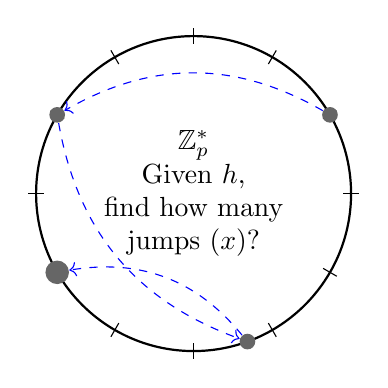
\begin{tikzpicture}
        % Clock
        \draw[thick] (0,0) circle (2cm);
        \foreach \angle in {0, 30, ..., 330} {
            \draw (\angle:1.9cm) -- (\angle:2.1cm);
        }
        
        % Jumps
        \node[circle, fill=blue, inner sep=2pt, label=right:$g^1$] (G1) at (30:2cm) {};
        \node[circle, fill=blue, inner sep=2pt, label=above:$g^2$] (G2) at (150:2cm) {};
        \node[circle, fill=blue, inner sep=2pt, label=below right:$g^3$] (G3) at (290:2cm) {};
        \node[circle, fill=red, inner sep=3pt, label=below left:\textbf{Target $h$}] (H) at (210:2cm) {};
        
        \draw[->, blue, dashed] (G1) to[bend right] (G2);
        \draw[->, blue, dashed] (G2) to[bend right] (G3);
        \draw[->, blue, dashed] (G3) to[bend right] (H);
        
        \node[align=center] at (0,0) {$\mathbb{Z}_p^*$\\Given $h$,\\find how many\\jumps ($x$)?};
    \end{tikzpicture}
    \caption{DLP behaves like determining the number of chaotic jumps on a clock face.}
\end{figure}

\subsection{The Elliptic Curve Discrete Logarithm Problem (ECDLP)}
This is the variant of the DLP used in ECDSA and ECDH. It operates on the algebraic structure of elliptic curves over finite fields.

\subsubsection*{Definition}
Given:
\begin{itemize}
    \item An elliptic curve $E$ defined over a finite field $\mathbb{F}_q$.
    \item A base point $P \in E(\mathbb{F}_q)$ of order $n$.
    \item A point $Q \in E(\mathbb{F}_q)$ (where $Q = k \cdot P$).
\end{itemize}
**The Problem:** Find the scalar integer $k$ such that:
\[ Q = \underbrace{P + P + \dots + P}_{k \text{ times}} \]

\subsubsection*{Why use Curves?}
The best known algorithms for solving classical DLP (like Index Calculus) do not work on general Elliptic Curves. The only known attacks are generic algorithms (like Pollard's rho) which have exponential time complexity $\mathcal{O}(\sqrt{n})$.
This allows ECDLP to achieve the same security level as RSA/DLP with \textbf{much smaller key sizes}.

\begin{figure}[H]
  \tikzset{
    concept/.style={circle, draw=blue!80!black, thick, fill=blue!5, align=center, minimum size=2.5cm, font=\bfseries},
    hard/.style={-Latex, very thick, red, dashed},
    easy/.style={-Latex, very thick, green!60!black},
    label/.style={midway, fill=white, font=\footnotesize, align=center}
}
    \centering
    \begin{tikzpicture}[scale=0.8]
        % Abstract Curve Visual
        \draw[thick, smooth, domain=-2:2.2, variable=\t] plot ({\t*2}, {0.5*\t^3 - 1.5*\t});
        
        \coordinate (P) at (-3, 0.5); % Just illustrative coords
        \coordinate (Q) at (3, 2);
        
        \node[circle, fill=blue, inner sep=2pt, label=above:$P$] at (P) {};
        \node[circle, fill=red, inner sep=2pt, label=right:$Q=kP$] at (Q) {};
        
        % Easy/Hard arrows
        \node[align=center] (Easy) at (0, -3) {\textbf{Point Multiplication}\\Given $k, P \to$ Compute $Q$\\ (Double-and-Add Algorithm)};
        \node[align=center] (Hard) at (0, -5) {\textbf{ECDLP}\\Given $Q, P \to$ Find $k$\\ (No sub-exponential algorithm)};
        
        \draw[easy] (-2, -3.5) -- (-2, -4.5);
        \draw[hard] (2, -4.5) -- (2, -3.5);
        
    \end{tikzpicture}
    \caption{ECDLP involves finding how many times $P$ was added to itself to reach $Q$.}
\end{figure}

\subsection{Security Comparison}
Approximate key sizes required for equivalent security levels (as per NIST recommendations).

\begin{table}[H]
    \centering
    \renewcommand{\arraystretch}{1.4}
    \begin{tabular}{@{} c c c c @{}}
        \toprule
        \textbf{Security Level} & \textbf{Symmetric Key} & \textbf{RSA / DLP Key} & \textbf{ECC Key} \\
        (Bits of Security) & (AES) & (Integer Factoring) & (ECDLP) \\
        \midrule
        80 & 80 bits & 1024 bits & 160 bits \\
        112 & 112 bits & 2048 bits & 224 bits \\
        128 & 128 bits & 3072 bits & 256 bits \\
        192 & 192 bits & 7680 bits & 384 bits \\
        256 & 256 bits & 15360 bits & 521 bits \\
        \bottomrule
    \end{tabular}
    \caption{Key Size Comparison. Notice how RSA keys must grow explosively to keep up, while ECC keys grow linearly.}
\end{table}


\subsection{RSA Encryption Scheme}
RSA is one of the first public-key cryptosystems and is widely used for secure data transmission. Unlike symmetric systems (like AES) which use the same key for encryption and decryption, RSA uses a pair of keys:
\begin{itemize}
    \item \textbf{Public Key}: Used to encrypt data. Can be shared openly.
    \item \textbf{Secret Key}: Used to decrypt data. Must be kept secret.
\end{itemize}

Key Sizes: 1024, 2048, 4092

RSA (Rivest-Shamir-Adleman) hardness is based on the prime factorization problem, since it is hard to factor the product of two large primes.

\subsubsection{Key Generation}

\begin{enumerate}
    \item \textbf{Prime Selection:} Choose two distinct large random primes $p, q$.
    \item \textbf{Modulus:} Compute $n = p \cdot q$.
    \item \textbf{Exponents:} Compute $\phi(n) = (p-1)(q-1)$. Select $e \in \mathbb{Z}_{\phi(n)}^*$ such that $\gcd(e, \phi(n)) = 1$. Compute $d \equiv e^{-1} \pmod{\phi(n)}$.
    \item \textbf{Output:} $pk = \langle n, e \rangle, \quad sk = \langle n, d \rangle$.
\end{enumerate}



\subsubsection{Encryption}

The encryption algorithm is deterministic (in textbook RSA) or probabilistic (in RSA-OAEP). Here we define textbook RSA.
\begin{itemize}
    \item \textbf{Input:} $pk = \langle n, e \rangle$, message $m \in \mathbb{Z}_n$.
    \item \textbf{Computation:} Compute ciphertext $c$:
    \[ c \equiv m^e \pmod n \]
    \item \textbf{Output:} $c \in \mathcal{C}$.
\end{itemize}

\begin{figure}[H]
    \centering
    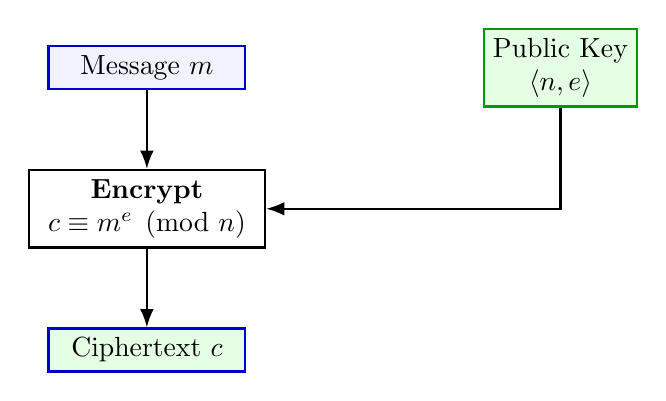
\begin{tikzpicture}[node distance=1.5cm]
        \node[data] (Msg) {Message $m$};
        \node[public, right=3cm of Msg] (PubKey) {Public Key\\$\langle n, e \rangle$};
        \node[op, below=1cm of Msg] (EncOp) {\textbf{Encrypt}\\$c \equiv m^e \pmod n$};
        \node[data, below=1cm of EncOp, fill=green!10] (Cipher) {Ciphertext $c$};
        
        \draw[arrow] (Msg) -- (EncOp);
        \draw[arrow] (PubKey) |- (EncOp);
        \draw[arrow] (EncOp) -- (Cipher);
    \end{tikzpicture}
    \caption{RSA Encryption $\mathsf{Enc}_{pk}(m)$.}
\end{figure}

\subsubsection{Decryption}

\begin{itemize}
    \item \textbf{Input:} $sk = \langle n, d \rangle$, ciphertext $c \in \mathbb{Z}_n$.
    \item \textbf{Computation:} Recover message $m'$:
    \[ m' \equiv c^d \pmod n \]
    \item \textbf{Output:} $m'$.
\end{itemize}


\subsubsection{Correctness Proof}

We must show that $\mathsf{Dec}_{sk}(\mathsf{Enc}_{pk}(m)) = m$.
Substituting the definition of $c$:
\[
c^d \equiv (m^e)^d \equiv m^{ed} \pmod n
\]
Since $ed \equiv 1 \pmod{\phi(n)}$, we have $ed = 1 + k\phi(n)$ for some integer $k$.
\[
m^{ed} \equiv m^{1 + k\phi(n)} \equiv m \cdot (m^{\phi(n)})^k \pmod n
\]
Assuming $m \in \mathbb{Z}_n^*$, by Euler's Theorem $m^{\phi(n)} \equiv 1 \pmod n$, so:
\[
m \cdot (1)^k \equiv m \pmod n
\]
(Note: The proof also holds for $m$ not in $\mathbb{Z}_n^*$ via the Chinese Remainder Theorem).


\subsection{ElGamal Encryption}

\textbf{ElGamal} is an asymmetric key encryption algorithm based on the \textbf{Diffie-Hellman Key Exchange}. Its security relies on the intractability of the \textbf{Discrete Logarithm Problem (DLP)}:

\begin{quote}
    Given $g, p,$ and $h = g^x \pmod p$, it is computationally hard to find $x$.
\end{quote}

A key feature of ElGamal is that it is \textbf{Probabilistic}: Encrypting the same message multiple times results in different ciphertexts.

\subsubsection{Key Generation $Gen$}

The algorithm takes a security parameter $1^\lambda$.
\begin{enumerate}
    \item \textbf{Group Generation:} Generate a cyclic group $\mathbb{G}$ of prime order $q$ with generator $g$.
    \item \textbf{Private Key:} Choose a random $x \leftarrow \mathbb{Z}_q$.
    \item \textbf{Public Key:} Compute $h = g^x$.
    \item \textbf{Output:} 
    \[ pk = \langle \mathbb{G}, q, g, h \rangle, \quad sk = \langle \mathbb{G}, q, g, x \rangle \]
\end{enumerate}



\subsubsection{Encryption $Enc$ (Alice)}

ElGamal is probabilistic. To encrypt $m \in \mathbb{G}$:
\begin{itemize}
    \item \textbf{Input:} $pk$, message $m$.
    \item \textbf{Randomness:} Choose an ephemeral key $y \leftarrow \mathbb{Z}_q$.
    \item \textbf{Computation:} Compute pair $(c_1, c_2)$:
    \[ c_1 = g^y, \quad c_2 = m \cdot h^y \]
    \item \textbf{Output:} Ciphertext $c = \langle c_1, c_2 \rangle$.
\end{itemize}

\begin{figure}[H]
    \centering
    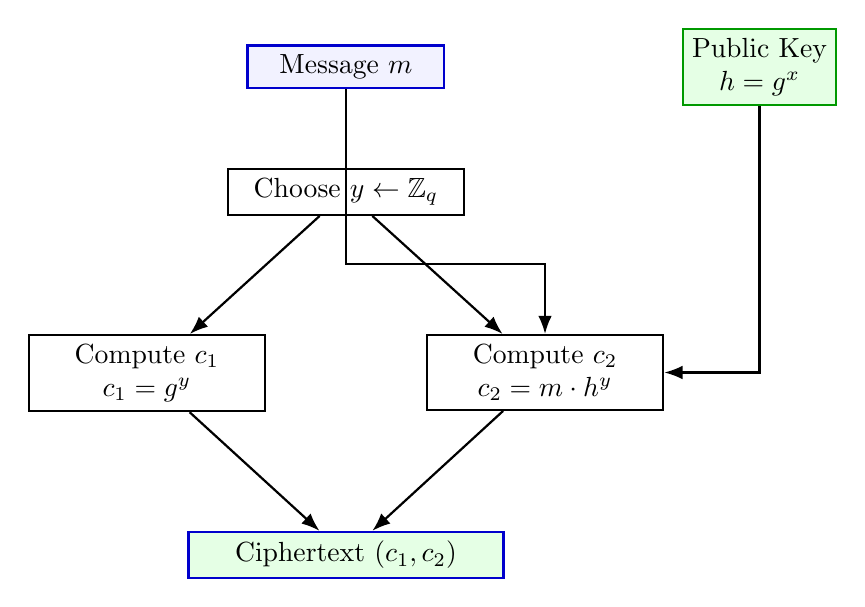
\begin{tikzpicture}[node distance=1.5cm]
        \node[data] (Msg) {Message $m$};
        \node[public, right=3cm of Msg] (PubKey) {Public Key\\$h = g^x$};
        \node[op, below=1cm of Msg] (Rand) {Choose $y \leftarrow \mathbb{Z}_q$};
        
        \node[op, below left=1.5cm and -0.5cm of Rand] (C1) {Compute $c_1$\\$c_1 = g^y$};
        \node[op, below right=1.5cm and -0.5cm of Rand] (C2) {Compute $c_2$\\$c_2 = m \cdot h^y$};
        
        \node[data, below=4cm of Rand, fill=green!10, minimum width=4cm] (Output) {Ciphertext $(c_1, c_2)$};
        
        \draw[arrow] (Msg) -- ++(0,-2.5) -| (C2);
        \draw[arrow] (PubKey) |- (C2);
        \draw[arrow] (Rand) -- (C1);
        \draw[arrow] (Rand) -- (C2);
        \draw[arrow] (C1) -- (Output);
        \draw[arrow] (C2) -- (Output);
    \end{tikzpicture}
    \caption{ElGamal Encryption $\mathsf{Enc}_{pk}(m)$.}
\end{figure}


\subsubsection{Decryption}

\begin{itemize}
    \item \textbf{Input:} $sk = x$, ciphertext $c = \langle c_1, c_2 \rangle$.
    \item \textbf{Computation:} Compute shared secret $s = c_1^x$. Then compute:
    \[ m' = c_2 \cdot s^{-1} \]
    \item \textbf{Output:} $m'$.
\end{itemize}

\begin{figure}[H]
    \centering
    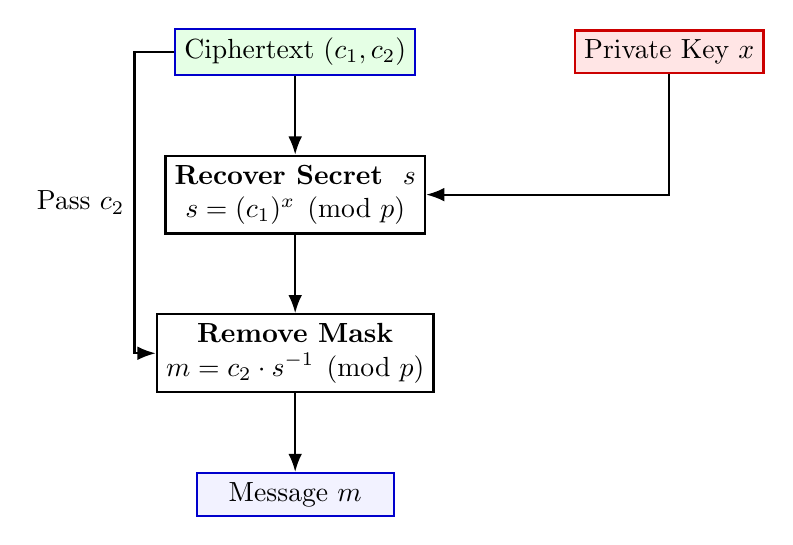
\begin{tikzpicture}[node distance=1.5cm]
        % Inputs
        \node[data, fill=green!10] (Input) {Ciphertext $(c_1, c_2)$};
        \node[secret, right=2cm of Input] (Priv) {Private Key $x$};
        
        % Step 1: Recover S
        \node[op, below=1cm of Input] (RecoverS) {\textbf{Recover Secret } $s$\\$s = (c_1)^x \pmod p$};
        
        % Step 2: Inverse
        \node[op, below=1cm of RecoverS] (Decrypt) {\textbf{Remove Mask}\\$m = c_2 \cdot s^{-1} \pmod p$};
        
        % Output
        \node[data, below=1cm of Decrypt] (Output) {Message $m$};
        
        % Wires
        \draw[arrow] (Input) -- (RecoverS);
        \draw[arrow] (Priv) |- (RecoverS);
        \draw[arrow] (RecoverS) -- (Decrypt);
        \draw[arrow] (Input.west) -- ++(-0.5,0) |- node[near start, left] {Pass $c_2$} (Decrypt.west);
        \draw[arrow] (Decrypt) -- (Output);

    \end{tikzpicture}
    \caption{Decryption Process. The math works because $(c_1)^x = (g^k)^x = g^{kx} = (g^x)^k = h^k = s$.}
\end{figure}

\subsubsection{Correctness Proof}
We show that $\mathsf{Dec}_{sk}(\mathsf{Enc}_{pk}(m)) = m$.
Substituting the values of $c_1$ and $c_2$:
\[
m' = c_2 \cdot (c_1^x)^{-1} = (m \cdot h^y) \cdot (g^y)^{-x}
\]
Since $h = g^x$:
\[
m' = (m \cdot (g^x)^y) \cdot (g^{yx})^{-1}
\]
\[
m' = m \cdot g^{xy} \cdot g^{-xy}
\]
\[
m' = m \cdot 1 = m
\]
Thus, the decryption correctly recovers the original message.

\subsubsection{Example}

Let's trace the values with small numbers.

\begin{enumerate}
    \item \textbf{Setup:}
    \begin{itemize}
        \item Prime $p = 23$, Generator $g = 5$.
        \item Bob chooses private $x = 6$.
        \item Bob computes $h = 5^6 \pmod{23} = 15625 \pmod{23} = 8$.
        \item Public Key: $(p=23, g=5, h=8)$.
    \end{itemize}
    
    \item \textbf{Encryption (Message $m = 10$):}
    \begin{itemize}
        \item Alice chooses random $k = 3$.
        \item Clue $c_1 = g^k = 5^3 = 125 \equiv 10 \pmod{23}$.
        \item Secret $s = h^k = 8^3 = 512 \equiv 6 \pmod{23}$.
        \item Mask $c_2 = m \cdot s = 10 \cdot 6 = 60 \equiv 14 \pmod{23}$.
        \item Ciphertext: $(10, 14)$.
    \end{itemize}
    
    \item \textbf{Decryption:}
    \begin{itemize}
        \item Bob receives $(10, 14)$.
        \item Recover $s = c_1^x = 10^6 \pmod{23} = 1000000 \pmod{23} = 6$. (Matches!).
        \item Find modular inverse of $6 \pmod{23}$. $6 \times 4 = 24 \equiv 1$. So $s^{-1} = 4$.
        \item $m = c_2 \cdot s^{-1} = 14 \cdot 4 = 56 \equiv 10 \pmod{23}$.
    \end{itemize}
\end{enumerate}

\section{Digital Signatures}

Digital signatures guarantee the non-repudation, integrity and authenticity properties. The algorithm is usually done agains the hash of $m$ message

A digital signature consists of three random, polinomial-time algorithms $(Gen, Sign, Vrfy)$, so:

\begin{itemize}
  \item \textbf{$Gen$ Key Generation Algorithm}: $Gen$ takes $1^n$ security parameter as input, and outputs $(pk, sk)$ keypair. We will refer to $pk$ as the public key and $sk$ as the secret key.
  We assume that $pk$ and $sk$ has a length of at least $n$, and $n$ can be defined from $(pk, sk)$ keypair. $(pk, sk) \leftarrow Gen(1^n) $
  \item \textbf{$Sign$ Signature Algorithm}: $Sign$ takes $sk$ secret key and message $m$ as inputs, and outputs signature $\sigma$. $\sigma \leftarrow Sign_{sk}(m)$
  \item \textbf{$Vrfy$ Verify Algorithm}: $Vrfy$ takes signature $\sigma$, public key $pk$ and $m$ as inputs, and outputs $b$ bit. If $b = 1$ the signature is valid, if $b = 0$ the signature is invalid. $b \leftarrow Vrfy_{pk}(\sigma, m) $ 
\end{itemize}


For all valid $m \in \mathcal{M}$ messages the following condition must satisfy: 
$Vrfy_{pk}(m,Sign_{sk}(m))=1$.


\subsection{RSA Signature Algorithm}

The RSA signature scheme is defined as a tuple of three probabilistic polynomial-time algorithms $(\mathsf{Gen}, \mathsf{Sign}, \mathsf{Vrfy})$ over a message space $\mathcal{M}$ and a signature space $\mathcal{S}$. We utilize a cryptographic hash function $H: \{0,1\}^* \to \mathbb{Z}_n$.


\subsubsection{Key Generation}


The key generation algorithm $\mathsf{Gen}$ takes a security parameter $1^\lambda$ as input and outputs a pair of keys $(pk, sk)$.

\begin{enumerate}
    \item \textbf{Prime Selection:} Choose two distinct large random primes $p, q$ of equal bit-length.
    \item \textbf{Modulus:} Compute $n = p \cdot q$. The group is defined over $\mathbb{Z}_n^*$.
    \item \textbf{Euler's Totient:} Compute $\phi(n) = (p-1)(q-1)$.
    \item \textbf{Public Exponent:} Select $e \in \mathbb{Z}_{\phi(n)}^*$ such that $\gcd(e, \phi(n)) = 1$.
    \item \textbf{Private Exponent:} Compute $d \equiv e^{-1} \pmod{\phi(n)}$.
    \item \textbf{Output:} 
    \[ pk = \langle n, e \rangle, \quad sk = \langle n, d \rangle \]
\end{enumerate}


\subsubsection{Signing Algorithm}

The signing algorithm takes the secret key $sk$ and a message $m \in \mathcal{M}$.

\begin{itemize}
    \item \textbf{Input:} $sk = \langle n, d \rangle$, message $m \in \{0,1\}^*$.
    \item \textbf{Hashing:} Compute the hash digest $h = H(m)$, where $h \in \mathbb{Z}_n$.
    \item \textbf{Computation:} Compute the signature $\sigma$ using the RSA primitive:
    \[ \sigma \equiv h^d \pmod n \]
    \item \textbf{Output:} The signature $\sigma \in \mathcal{S}$.
\end{itemize}

\begin{figure}[H]
    \centering
    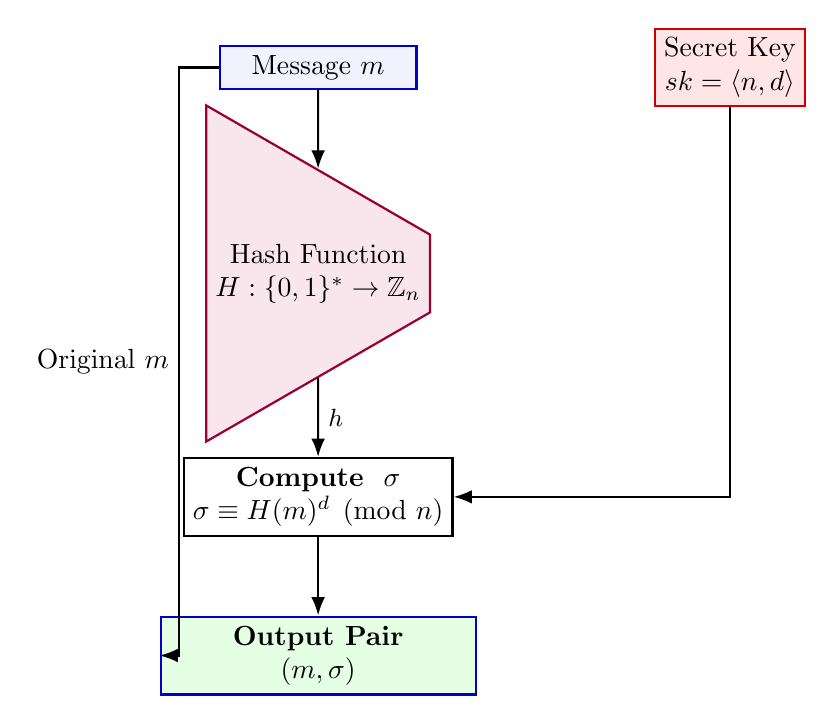
\begin{tikzpicture}[node distance=1.5cm]
        % Inputs
        \node[data] (Msg) {Message $m$};
        \node[secret, right=3cm of Msg] (PrivKey) {Secret Key\\$sk = \langle n, d \rangle$};
        
        % Hash Step
        \node[hash, below=1cm of Msg] (HashFunc) {Hash Function\\$H: \{0,1\}^* \to \mathbb{Z}_n$};
        
        % Signing Step (Math)
        \node[op, below=1cm of HashFunc] (SignOp) {\textbf{Compute } $\sigma$\\$\sigma \equiv H(m)^d \pmod n$};
        
        % Output
        \node[data, below=1cm of SignOp, fill=green!10, minimum width=4cm] (Package) {\textbf{Output Pair}\\$(m, \sigma)$};
        
        % Connections
        \draw[arrow] (Msg) -- (HashFunc);
        \draw[arrow] (HashFunc) -- node[right, font=\small] {$h$} (SignOp);
        \draw[arrow] (PrivKey) |- (SignOp);
        
        \draw[arrow] (SignOp) -- (Package);
        \draw[arrow] (Msg.west) -- ++(-0.5,0) |- node[near start, left] {Original $m$} (Package.west);

    \end{tikzpicture}
    \caption{The Signing Algorithm $\mathsf{Sign}_{sk}(m)$.}
\end{figure}

\subsubsection{Verification Algorithm}

The verification algorithm is deterministic. It takes the public key $pk$, a message $m$, and a signature $\sigma$. It outputs a bit $b \in \{0, 1\}$ (1 for valid, 0 for invalid).

\begin{itemize}
    \item \textbf{Input:} $pk = \langle n, e \rangle$, message $m$, signature $\sigma$.
    \item \textbf{Hashing:} Compute $h = H(m)$.
    \item \textbf{Inversion:} Compute $h' \equiv \sigma^e \pmod n$.
    \item \textbf{Check:} Verify if $h' \stackrel{?}{=} h$.
    \[
    \mathsf{Vrfy}_{pk}(m, \sigma) = 
    \begin{cases} 
    1 & \text{if } \sigma^e \equiv H(m) \pmod n \\
    0 & \text{otherwise}
    \end{cases}
    \]
\end{itemize}

\begin{figure}[H]
    \centering
    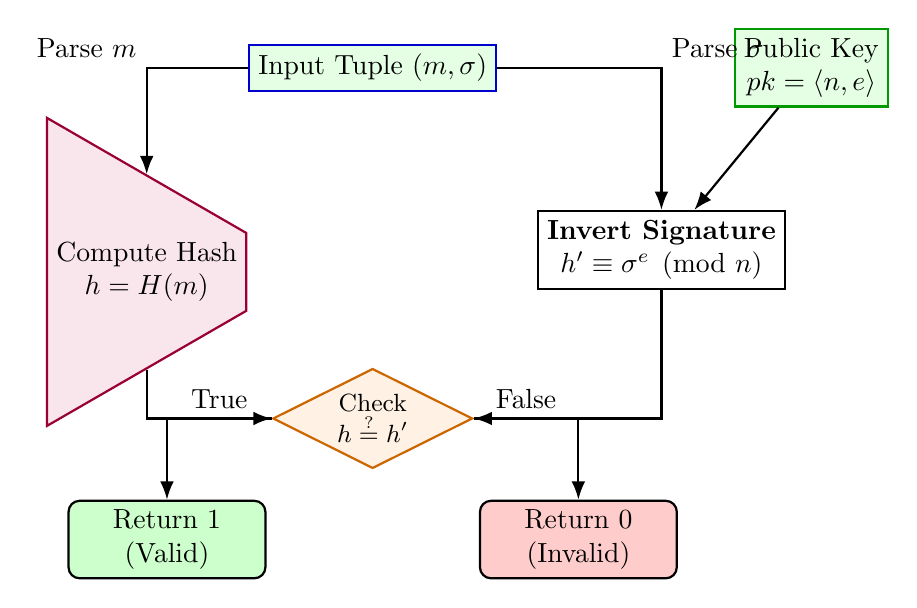
\begin{tikzpicture}[node distance=1.5cm]
        % Input Package
        \node[data, fill=green!10] (Input) {Input Tuple $(m, \sigma)$};
        \node[public, right=3cm of Input] (PubKey) {Public Key\\$pk = \langle n, e \rangle$};
        
        % Path 1: Process Message
        \node[hash, below left=1.5cm and 0.5cm of Input] (ReHash) {Compute Hash\\$h = H(m)$};
        
        % Path 2: Process Signature
        \node[op, below right=1.5cm and 0.5cm of Input] (Unsign) {\textbf{Invert Signature}\\$h' \equiv \sigma^e \pmod n$};
        
        % Comparison
        \node[check, below=3.5cm of Input] (Compare) {Check\\$h \stackrel{?}{=} h'$};
        
        % Outcomes
        \node[sigStep, below left=1cm of Compare, fill=green!20, minimum width=2.5cm] (Valid) {Return 1\\(Valid)};
        \node[sigStep, below right=1cm of Compare, fill=red!20, minimum width=2.5cm] (Invalid) {Return 0\\(Invalid)};
        
        % Connections
        \draw[arrow] (Input) -| node[above left] {Parse $m$} (ReHash);
        \draw[arrow] (Input) -| node[above right] {Parse $\sigma$} (Unsign);
        \draw[arrow] (PubKey) -- (Unsign);
        
        \draw[arrow] (ReHash) |- (Compare);
        \draw[arrow] (Unsign) |- (Compare);
        
        \draw[arrow] (Compare) -| node[above, near start] {True} (Valid);
        \draw[arrow] (Compare) -| node[above, near start] {False} (Invalid);

    \end{tikzpicture}
    \caption{The Verification Algorithm $\mathsf{Vrfy}_{pk}(m, \sigma)$.}
\end{figure}

\subsubsection{Correctness Proof}

We must show that for any valid signature generated by $\mathsf{Sign}$, $\mathsf{Vrfy}$ returns 1.

Given $\sigma \equiv h^d \pmod n$ where $h = H(m)$, the verifier computes $\sigma^e \pmod n$.
Using Euler's Theorem, since $ed \equiv 1 \pmod{\phi(n)}$, we have $ed = k\phi(n) + 1$ for some integer $k$.

\[
\sigma^e \equiv (h^d)^e \equiv h^{de} \equiv h^{k\phi(n) + 1} \equiv (h^{\phi(n)})^k \cdot h \pmod n
\]

Since $h \in \mathbb{Z}_n^*$, by Euler's Theorem $h^{\phi(n)} \equiv 1 \pmod n$. Thus:
\[
1^k \cdot h \equiv h \pmod n
\]
Therefore, $\sigma^e \equiv H(m) \pmod n$, and the verification succeeds.

\subsection{DSA Signature Scheme}

The Digital Signature Algorithm (DSA) is a FIPS standard (FIPS 186) based on the discrete logarithm problem. It is defined as a tuple $(\mathsf{Gen}, \mathsf{Sign}, \mathsf{Vrfy})$ utilizing a cryptographic hash function $H: \{0,1\}^* \to \mathbb{Z}_q$.

\subsubsection{Key Generation ($\mathsf{Gen}$)}
The key generation algorithm takes security parameters $L$ and $N$ (e.g., $L=2048, N=256$).

\begin{enumerate}
    \item \textbf{Parameter Generation:}
    \begin{itemize}
        \item Choose a prime $q$ of length $N$ bits.
        \item Choose a prime $p$ of length $L$ bits such that $p - 1$ is a multiple of $q$.
        \item Choose an integer $h$ ($1 < h < p-1$) such that $g = h^{(p-1)/q} \bmod p > 1$.
        \item $(p, q, g)$ are public domain parameters.
    \end{itemize}
    \item \textbf{Private Key:} Choose a random integer $x$ such that $0 < x < q$.
    \item \textbf{Public Key:} Compute $y = g^x \bmod p$.
    \item \textbf{Output:} 
    \[ pk = \langle p, q, g, y \rangle, \quad sk = \langle p, q, g, x \rangle \]
\end{enumerate}

\subsubsection{Signing Algorithm ($\mathsf{Sign}$)}
The signing algorithm is probabilistic. It takes the secret key $sk$ and a message $m$.

\begin{itemize}
    \item \textbf{Input:} $sk$, message $m$.
    \item \textbf{Nonce Generation:} Choose a random per-message integer $k$ such that $0 < k < q$.
    \item \textbf{Computation:}
    \begin{enumerate}
        \item Compute $r = (g^k \bmod p) \bmod q$.
        \item Compute $z = H(m)$ (taking the leftmost $\min(N, \text{outlen})$ bits).
        \item Compute $s = k^{-1}(z + x \cdot r) \bmod q$.
    \end{enumerate}
    \item \textbf{Retry:} If $r=0$ or $s=0$, restart with a new $k$.
    \item \textbf{Output:} Signature $\sigma = (r, s)$.
\end{itemize}

\begin{figure}[H]
    \centering
    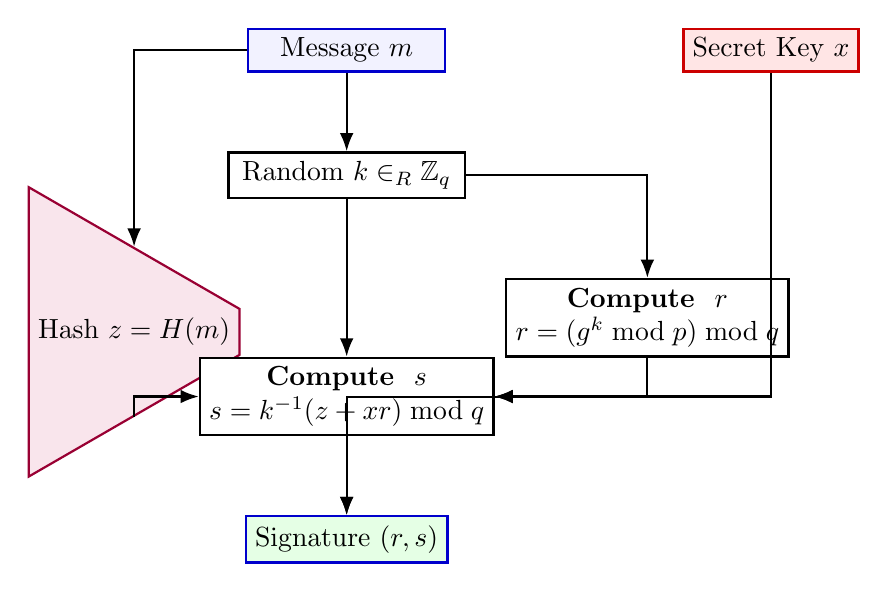
\begin{tikzpicture}[node distance=1.5cm]
        % Inputs
        \node[data] (Msg) {Message $m$};
        \node[secret, right=3cm of Msg] (PrivKey) {Secret Key $x$};
        \node[op, below=1cm of Msg] (Rand) {Random $k \in_R \mathbb{Z}_q$};
        
        % Hash
        \node[hash, below left=1cm and 0.5cm of Rand] (Hash) {Hash $z = H(m)$};
        
        % Math Steps
        \node[op, below right=1cm and 0.5cm of Rand] (CalcR) {\textbf{Compute } $r$\\$r = (g^k \bmod p) \bmod q$};
        
        \node[op, below=2cm of Rand] (CalcS) {\textbf{Compute } $s$\\$s = k^{-1}(z + xr) \bmod q$};
        
        % Output
        \node[data, below=1cm of CalcS, fill=green!10] (Sig) {Signature $(r, s)$};
        
        % Connections
        \draw[arrow] (Msg) -- (Rand); % Abstract flow
        \draw[arrow] (Msg) -| (Hash);
        \draw[arrow] (Rand) -| (CalcR);
        \draw[arrow] (Rand) -- (CalcS);
        \draw[arrow] (Hash) |- (CalcS);
        \draw[arrow] (CalcR) |- (CalcS);
        \draw[arrow] (PrivKey) |- (CalcS);
        
        \draw[arrow] (CalcS) -- (Sig);
        % Include r in signature
        \draw[arrow] (CalcR.south) -- ++(0,-0.5) -| (Sig.north);

    \end{tikzpicture}
    \caption{DSA Signing Process $\mathsf{Sign}_{sk}(m)$.}
\end{figure}

\subsubsection{Verification Algorithm ($\mathsf{Vrfy}$)}
The verification algorithm takes the public key $pk$, message $m$, and signature $\sigma=(r, s)$.

\begin{itemize}
    \item \textbf{Check:} Verify $0 < r < q$ and $0 < s < q$. If not, return Invalid.
    \item \textbf{Computation:}
    \begin{enumerate}
        \item Compute $w = s^{-1} \bmod q$.
        \item Compute hash $z = H(m)$.
        \item Compute $u_1 = z \cdot w \bmod q$.
        \item Compute $u_2 = r \cdot w \bmod q$.
        \item Compute $v = (g^{u_1} y^{u_2} \bmod p) \bmod q$.
    \end{enumerate}
    \item \textbf{Output:} Valid if $v = r$, otherwise Invalid.
\end{itemize}

\begin{figure}[H]
    \centering
    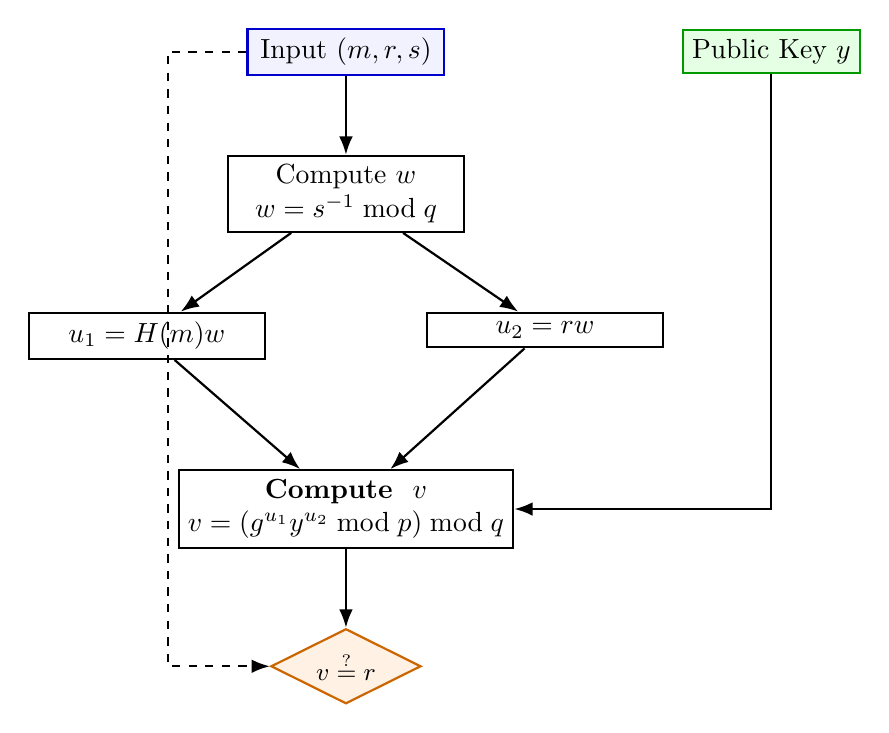
\begin{tikzpicture}[node distance=1.5cm]
        \node[data] (Input) {Input $(m, r, s)$};
        \node[public, right=3cm of Input] (PubKey) {Public Key $y$};
        
        \node[op, below=1cm of Input] (Invert) {Compute $w$\\$w = s^{-1} \bmod q$};
        
        \node[op, below left=1cm and -0.5cm of Invert] (U1) {$u_1 = H(m)w$};
        \node[op, below right=1cm and -0.5cm of Invert] (U2) {$u_2 = rw$};
        
        \node[op, below=3cm of Invert] (CalcV) {\textbf{Compute } $v$\\$v = (g^{u_1}y^{u_2} \bmod p) \bmod q$};
        
        \node[check, below=1cm of CalcV] (Check) {$v \stackrel{?}{=} r$};
        
        \draw[arrow] (Input) -- (Invert);
        \draw[arrow] (Invert) -- (U1);
        \draw[arrow] (Invert) -- (U2);
        \draw[arrow] (U1) -- (CalcV);
        \draw[arrow] (U2) -- (CalcV);
        \draw[arrow] (PubKey) |- (CalcV);
        \draw[arrow] (CalcV) -- (Check);
        
        % Pass r down
        \draw[arrow, dashed] (Input.west) -- ++(-1,0) |- (Check.west);
    \end{tikzpicture}
    \caption{DSA Verification Process $\mathsf{Vrfy}_{pk}(m, \sigma)$.}
\end{figure}

\subsubsection{Correctness Proof}
We show that if the signature is valid, then $v = r$.
Recall $s \equiv k^{-1}(z + xr) \pmod q$. Thus $k \equiv s^{-1}(z + xr) \pmod q$.
Substituting $w = s^{-1}$:
\[
k \equiv w(z + xr) \equiv zw + xrw \equiv u_1 + x u_2 \pmod q
\]
Therefore, we can write $k = u_1 + x u_2 + nq$ for some integer $n$.
Now compute $v$:
\[
v = (g^{u_1} y^{u_2} \bmod p) \bmod q
\]
Substitute $y = g^x$:
\[
v = (g^{u_1} (g^x)^{u_2} \bmod p) \bmod q = (g^{u_1 + x u_2} \bmod p) \bmod q
\]
Since $g$ has order $q$ modulo $p$ (i.e., $g^q \equiv 1 \pmod p$), the exponent works modulo $q$:
\[
g^{u_1 + x u_2} \equiv g^{k - nq} \equiv g^k \cdot (g^q)^{-n} \equiv g^k \cdot 1^{-n} \equiv g^k \pmod p
\]
Thus:
\[
v = (g^k \bmod p) \bmod q
\]
By definition of the signing algorithm, $r = (g^k \bmod p) \bmod q$.
Therefore, $v = r$.

\section{Elliptik Curve Digital Signature ALgorithm Scheme (ECDSA)}

\section{Formal Definition}
ECDSA is an ANSI, FIPS, and IEEE standard. It operates in an elliptic curve group $\mathbb{E}(\mathbb{F}_q)$ rather than the multiplicative group of integers used in DSA. It is defined as a tuple $(\mathsf{Gen}, \mathsf{Sign}, \mathsf{Vrfy})$.

\section{1. Key Generation ($\mathsf{Gen}$)}
The algorithm takes a security parameter defining the curve parameters.

\begin{enumerate}
    \item \textbf{Domain Parameters:}
    \begin{itemize}
        \item An elliptic curve $E$ defined over a finite field $\mathbb{F}_q$.
        \item A base point $G \in E(\mathbb{F}_q)$ of large prime order $n$.
        \item The order $n$ (where $n \times G = \mathcal{O}$, the point at infinity).
    \end{itemize}
    \item \textbf{Private Key:} Choose a random integer $d$ such that $1 \le d \le n-1$.
    \item \textbf{Public Key:} Compute the point $Q = d \times G$ (Scalar Multiplication).
    \item \textbf{Output:} 
    \[ pk = \langle E, G, n, Q \rangle, \quad sk = \langle E, G, n, d \rangle \]
\end{enumerate}

\subsubsection{Signing Algorithm ($\mathsf{Sign}$)}
To sign a message $m$:

\begin{itemize}
    \item \textbf{Input:} $sk$, message $m$.
    \item \textbf{Nonce:} Select a random integer $k \in_R [1, n-1]$.
    \item \textbf{Computation:}
    \begin{enumerate}
        \item Compute point $R = k \times G = (x_1, y_1)$.
        \item Compute $r = x_1 \pmod n$. (If $r=0$, try new $k$).
        \item Compute hash $z = H(m)$ (truncated to bit-length of $n$).
        \item Compute $s = k^{-1}(z + r \cdot d) \pmod n$. (If $s=0$, try new $k$).
    \end{enumerate}
    \item \textbf{Output:} Signature $\sigma = (r, s)$.
\end{itemize}

\begin{figure}[H]
    \centering
    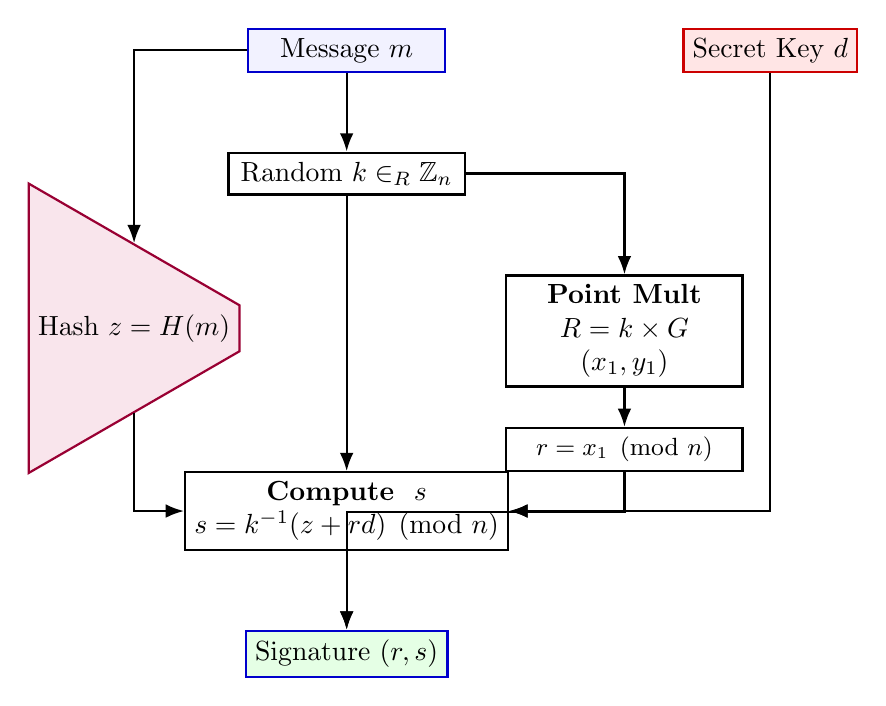
\begin{tikzpicture}[node distance=1.5cm]
        % Inputs
        \node[data] (Msg) {Message $m$};
        \node[secret, right=3cm of Msg] (PrivKey) {Secret Key $d$};
        \node[op, below=1cm of Msg] (Rand) {Random $k \in_R \mathbb{Z}_n$};
        
        % Hash
        \node[hash, below left=1cm and 0.5cm of Rand] (Hash) {Hash $z = H(m)$};
        
        % Point Mult Step
        \node[op, below right=1cm and 0.5cm of Rand] (PointMult) {\textbf{Point Mult}\\$R = k \times G$\\$(x_1, y_1)$};
        
        % Scalar Math
        \node[op, below=3.5cm of Rand] (CalcS) {\textbf{Compute } $s$\\$s = k^{-1}(z + rd) \pmod n$};
        
        % Coordinate extraction
        \node[op, below=0.5cm of PointMult, font=\small] (Extract) {$r = x_1 \pmod n$};
        
        % Output
        \node[data, below=1cm of CalcS, fill=green!10] (Sig) {Signature $(r, s)$};
        
        % Connections
        \draw[arrow] (Msg) -- (Rand); % Abstract flow
        \draw[arrow] (Msg) -| (Hash);
        \draw[arrow] (Rand) -| (PointMult);
        \draw[arrow] (Rand) -- (CalcS);
        \draw[arrow] (PointMult) -- (Extract);
        
        \draw[arrow] (Hash) |- (CalcS);
        \draw[arrow] (Extract) |- (CalcS);
        \draw[arrow] (PrivKey) |- (CalcS);
        
        \draw[arrow] (CalcS) -- (Sig);
        \draw[arrow] (Extract.south) -- ++(0,-0.5) -| (Sig.north);

    \end{tikzpicture}
    \caption{ECDSA Signing Process $\mathsf{Sign}_{sk}(m)$.}
\end{figure}

\subsubsection{Verification Algorithm ($\mathsf{Vrfy}$)}
To verify signature $\sigma=(r, s)$ for message $m$:

\begin{itemize}
    \item \textbf{Check:} Verify $r, s \in [1, n-1]$.
    \item \textbf{Computation:}
    \begin{enumerate}
        \item Compute $w = s^{-1} \pmod n$.
        \item Compute hash $z = H(m)$.
        \item Compute $u_1 = z \cdot w \pmod n$.
        \item Compute $u_2 = r \cdot w \pmod n$.
        \item Compute point $P = u_1 \times G + u_2 \times Q$. (Check if $P = \mathcal{O}$).
        \item Extract $P = (x_P, y_P)$.
        \item Compute $v = x_P \pmod n$.
    \end{enumerate}
    \item \textbf{Output:} Valid if $v = r$, otherwise Invalid.
\end{itemize}

\begin{figure}[H]
    \centering
    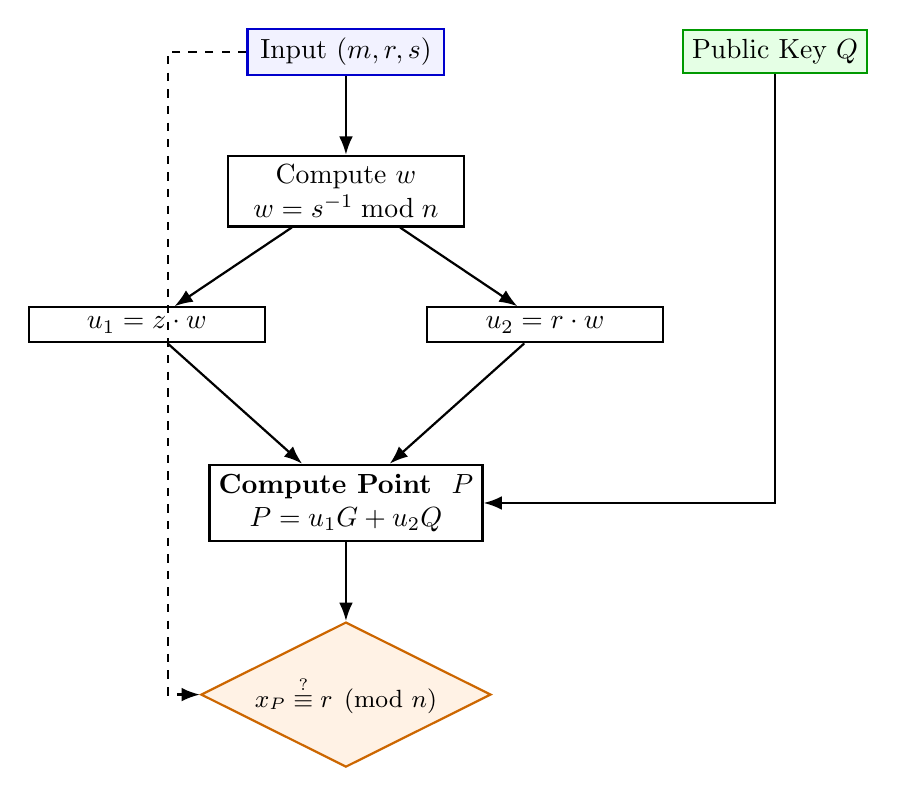
\begin{tikzpicture}[node distance=1.5cm]
        \node[data] (Input) {Input $(m, r, s)$};
        \node[public, right=3cm of Input] (PubKey) {Public Key $Q$};
        
        \node[op, below=1cm of Input] (Invert) {Compute $w$\\$w = s^{-1} \bmod n$};
        
        \node[op, below left=1cm and -0.5cm of Invert] (U1) {$u_1 = z \cdot w$};
        \node[op, below right=1cm and -0.5cm of Invert] (U2) {$u_2 = r \cdot w$};
        
        \node[op, below=3cm of Invert] (CalcP) {\textbf{Compute Point } $P$\\$P = u_1 G + u_2 Q$};
        
        \node[check, below=1cm of CalcP] (Check) {$x_P \stackrel{?}{\equiv} r \pmod n$};
        
        \draw[arrow] (Input) -- (Invert);
        \draw[arrow] (Invert) -- (U1);
        \draw[arrow] (Invert) -- (U2);
        \draw[arrow] (U1) -- (CalcP);
        \draw[arrow] (U2) -- (CalcP);
        \draw[arrow] (PubKey) |- (CalcP);
        \draw[arrow] (CalcP) -- (Check);
        
        % Pass r down
        \draw[arrow, dashed] (Input.west) -- ++(-1,0) |- (Check.west);
    \end{tikzpicture}
    \caption{ECDSA Verification Process $\mathsf{Vrfy}_{pk}(m, \sigma)$.}
\end{figure}

\subsubsection{Correctness Proof}
We verify that the calculated point $P$ essentially reconstructs the random point $R$ used during signing.

Recall $s \equiv k^{-1}(z + rd) \pmod n$. Thus $k \equiv s^{-1}(z + rd) \pmod n$.
Substituting $w = s^{-1}$:
\[
k \equiv w(z + rd) \equiv z w + r d w \equiv u_1 + u_2 d \pmod n
\]
Therefore:
\[
k \times G = (u_1 + u_2 d) \times G = u_1 \times G + u_2 \times (d \times G)
\]
Since $Q = d \times G$, we have:
\[
k \times G = u_1 \times G + u_2 \times Q
\]
Thus, the verification point $P$ is exactly the original point $R$ (where $R = k \times G$).
Consequently, $x_P \equiv x_1 \equiv r \pmod n$.


\section{Key excahnge algorithms}

\subsection{RSA Key Transport (Key Exchange)}
Unlike Diffie-Hellman, RSA Key Transport is asymmetric: one party defines the key, encrypts it, and sends it to the other.

\subsubsection{Setup}
\begin{itemize}
    \item \textbf{Bob (Receiver):} Generates RSA keys.
    \begin{itemize}
        \item Public Key: $(n, e)$.
        \item Private Key: $(n, d)$.
    \end{itemize}
\end{itemize}

\subsubsection{Protocol Flow}
\begin{enumerate}
    \item \textbf{Bob:} Sends Public Key $(n, e)$ to Alice.
    \item \textbf{Alice (Initiator):} 
    \begin{itemize}
        \item Generates a random session key $K$ (e.g., 256 bits).
        \item Converts $K$ to integer $m$ (with padding, e.g., PKCS\#1 v1.5 or OAEP).
        \item Computes ciphertext $c \equiv m^e \pmod n$.
        \item Sends $c$ to Bob.
    \end{itemize}
    \item \textbf{Bob:}
    \begin{itemize}
        \item Decrypts $m \equiv c^d \pmod n$.
        \item Extracts $K$ from the padded message $m$.
    \end{itemize}
\end{enumerate}

\begin{figure}[H]
    \centering
    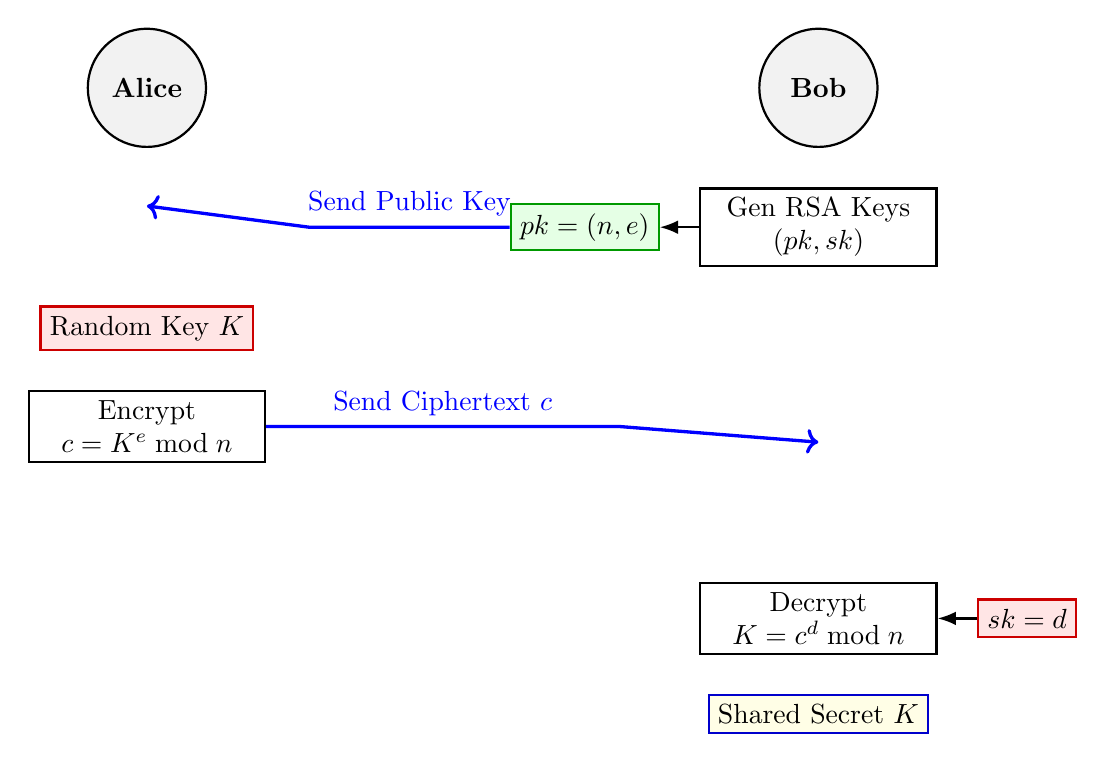
\begin{tikzpicture}[node distance=1.5cm]
        \node[actor] (Alice) {Alice};
        \node[actor, right=7cm of Alice] (Bob) {Bob};
        
        % Bob generates keys
        \node[op, below=0.5cm of Bob] (Gen) {Gen RSA Keys\\$(pk, sk)$};
        \node[public, left=0.5cm of Gen] (Pub) {$pk=(n,e)$};
        \draw[arrow] (Gen) -- (Pub);
        
        % Bob sends PK
        \draw[->, very thick, blue] (Pub) -- node[above] {Send Public Key} ($(Pub)-(3.5,0)$) -- ($(Alice)+(0,-1.5)$);
        
        % Alice operations
        \node[secret, below=2cm of Alice] (K) {Random Key $K$};
        \node[op, below=0.5cm of K] (Enc) {Encrypt\\$c = K^e \bmod n$};
        
        % Alice sends Ciphertext
        \draw[->, very thick, blue] (Enc) -- node[above] {Send Ciphertext $c$} ($(Enc)+(6,0)$) -- ($(Bob)+(0,-4.5)$);
        
        % Bob decrypts
        \node[op, below=4cm of Gen] (Dec) {Decrypt\\$K = c^d \bmod n$};
        \node[secret, right=0.5cm of Dec] (Sk) {$sk=d$};
        
        \draw[arrow] (Sk) -- (Dec);
        
        % Result
        \node[data, below=0.5cm of Dec, fill=yellow!10] (Result) {Shared Secret $K$};
        
    \end{tikzpicture}
    \caption{RSA Key Transport Protocol.}
\end{figure}



\subsection{Diffie-Hellman Key Exchange (DHKE)}
A protocol allowing two parties to jointly establish a shared secret over an insecure channel.

\subsubsection{Setup}
\begin{itemize}
    \item \textbf{Parameters:} A large prime $p$ and a generator $g$ of the multiplicative group $\mathbb{Z}_p^*$.
\end{itemize}

\subsubsection{Protocol Flow}
\begin{enumerate}
    \item \textbf{Alice:} Chooses secret integer $a \in_R [1, p-2]$. Computes $A = g^a \pmod p$. Sends $A$ to Bob.
    \item \textbf{Bob:} Chooses secret integer $b \in_R [1, p-2]$. Computes $B = g^b \pmod p$. Sends $B$ to Alice.
    \item \textbf{Key Computation:}
    \begin{itemize}
        \item Alice computes $S_A = B^a \pmod p$.
        \item Bob computes $S_B = A^b \pmod p$.
    \end{itemize}
    \item \textbf{Shared Secret:} $K = S_A = S_B$.
\end{enumerate}

\begin{figure}[H]
    \centering
    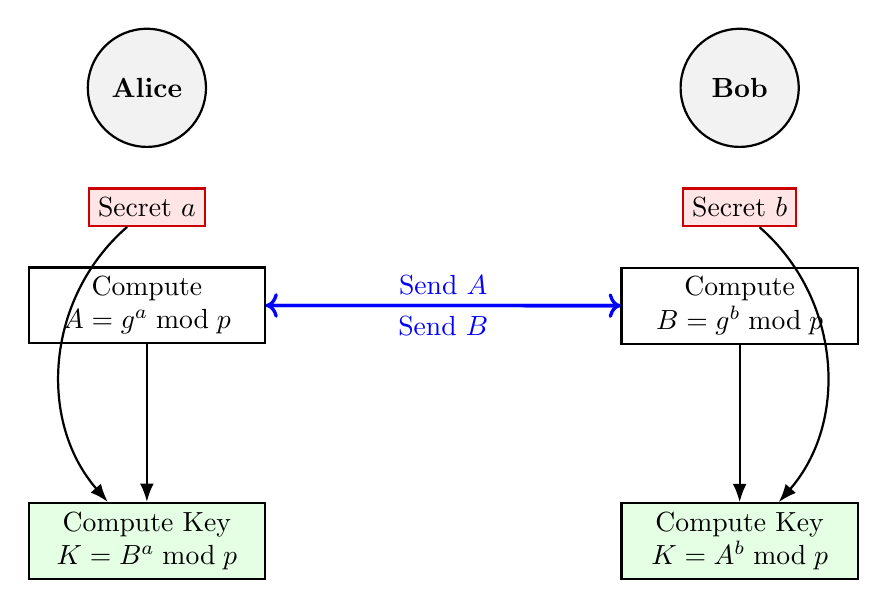
\begin{tikzpicture}[node distance=1.5cm, auto]
        % Actors
        \node[actor] (Alice) {Alice};
        \node[actor, right=6cm of Alice] (Bob) {Bob};
        
        % Alice Ops
        \node[secret, below=0.5cm of Alice] (SecA) {Secret $a$};
        \node[op, below=0.5cm of SecA] (CalcA) {Compute\\$A = g^a \bmod p$};
        
        % Bob Ops
        \node[secret, below=0.5cm of Bob] (SecB) {Secret $b$};
        \node[op, below=0.5cm of SecB] (CalcB) {Compute\\$B = g^b \bmod p$};
        
        % Exchange
        \draw[->, very thick, blue] (CalcA) -- node[above] {Send $A$} (CalcB);
        \draw[->, very thick, blue] (CalcB) -- node[below] {Send $B$} (CalcA);
        
        % Final Computation
        \node[op, below=2cm of CalcA, fill=green!10] (KeyA) {Compute Key\\$K = B^a \bmod p$};
        \node[op, below=2cm of CalcB, fill=green!10] (KeyB) {Compute Key\\$K = A^b \bmod p$};
        
        \draw[arrow] (CalcA) -- (KeyA);
        \draw[arrow] (CalcB) -- (KeyB);
        \draw[arrow] (SecA) to[bend right=45] (KeyA);
        \draw[arrow] (SecB) to[bend left=45] (KeyB);
    \end{tikzpicture}
    \caption{Diffie-Hellman Key Exchange.}
\end{figure}

\subsubsection{Correctness Proof}
\[
S_A \equiv B^a \equiv (g^b)^a \equiv g^{ba} \pmod p
\]
\[
S_B \equiv A^b \equiv (g^a)^b \equiv g^{ab} \pmod p
\]
Since multiplication in the exponent is commutative ($ab = ba$), $S_A = S_B$.

\subsection{Elliptic Curve Diffie-Hellman (ECDH)}
An variant of DHKE using additive elliptic curve groups, offering smaller key sizes for equivalent security.

\subsubsection{Setup}
\begin{itemize}
    \item \textbf{Parameters:} Elliptic curve $E(\mathbb{F}_q)$, base point $G$ of order $n$.
\end{itemize}

\subsubsection{Protocol Flow}
\begin{enumerate}
    \item \textbf{Alice:} Chooses private $d_A \in_R [1, n-1]$. Computes public point $Q_A = d_A \times G$.
    \item \textbf{Bob:} Chooses private $d_B \in_R [1, n-1]$. Computes public point $Q_B = d_B \times G$.
    \item \textbf{Exchange:} Parties exchange $Q_A$ and $Q_B$.
    \item \textbf{Key Derivation:}
    \begin{itemize}
        \item Alice computes point $S = d_A \times Q_B$.
        \item Bob computes point $S = d_B \times Q_A$.
    \end{itemize}
    \item \textbf{Shared Secret:} The x-coordinate of $S$, denoted $x_S$, is the shared secret.
\end{enumerate}

\begin{figure}[H]
    \centering
    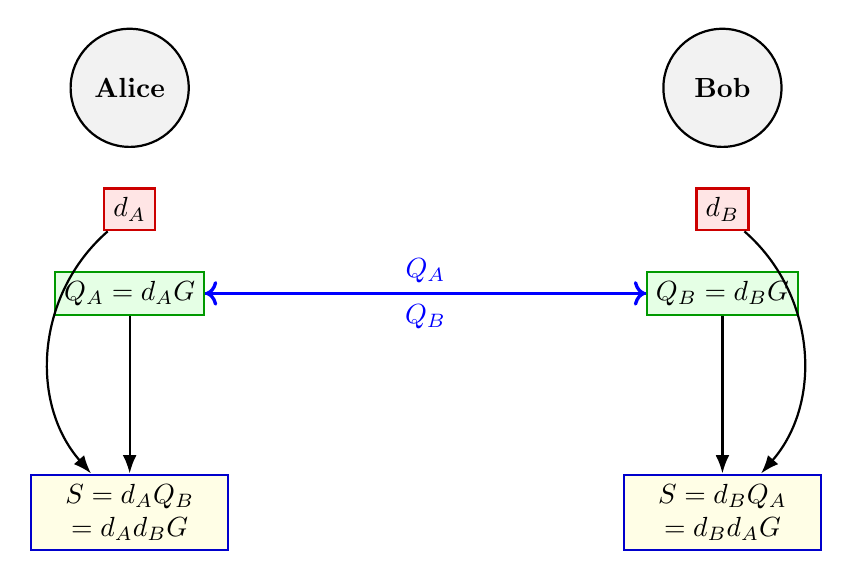
\begin{tikzpicture}[node distance=1.5cm, auto]
        \node[actor] (Alice) {Alice};
        \node[actor, right=6cm of Alice] (Bob) {Bob};
        
        % Private Keys
        \node[secret, below=0.5cm of Alice] (PrivA) {$d_A$};
        \node[secret, below=0.5cm of Bob] (PrivB) {$d_B$};
        
        % Public Keys
        \node[public, below=0.5cm of PrivA] (PubA) {$Q_A = d_A G$};
        \node[public, below=0.5cm of PrivB] (PubB) {$Q_B = d_B G$};
        
        % Exchange
        \draw[->, very thick, blue] (PubA) -- node[above] {$Q_A$} (PubB);
        \draw[->, very thick, blue] (PubB) -- node[below] {$Q_B$} (PubA);
        
        % Shared Secret
        \node[data, below=2cm of PubA, fill=yellow!10] (SecretA) {$S = d_A Q_B$\\$= d_A d_B G$};
        \node[data, below=2cm of PubB, fill=yellow!10] (SecretB) {$S = d_B Q_A$\\$= d_B d_A G$};
        
        \draw[arrow] (PubA) -- (SecretA);
        \draw[arrow] (PubB) -- (SecretB);
        \draw[arrow] (PrivA) to[bend right=45] (SecretA);
        \draw[arrow] (PrivB) to[bend left=45] (SecretB);
    \end{tikzpicture}
    \caption{ECDH Protocol Flow.}
\end{figure}

\subsubsection{Correctness Proof}
\[
S_{Alice} = d_A \times Q_B = d_A \times (d_B \times G) = (d_A \cdot d_B) \times G
\]
\[
S_{Bob} = d_B \times Q_A = d_B \times (d_A \times G) = (d_B \cdot d_A) \times G
\]
Since scalar multiplication is associative and commutative over scalars, the points are identical.


\section{Cryptographic Hash Functions}

\subsection{Formal Definition}
A cryptographic hash function is a deterministic algorithm $H: \{0,1\}^* \to \{0,1\}^n$ that maps an arbitrary length input $m$ to a fixed length output $h = H(m)$. It must satisfy three core security properties:
\begin{enumerate}
    \item \textbf{Pre-image Resistance:} Given $h$, it is computationally infeasible to find $m$ such that $H(m) = h$.
    \item \textbf{Second Pre-image Resistance:} Given $m_1$, it is infeasible to find $m_2 \neq m_1$ such that $H(m_1) = H(m_2)$.
    \item \textbf{Collision Resistance:} It is infeasible to find any pair $m_1 \neq m_2$ such that $H(m_1) = H(m_2)$.
\end{enumerate}

\subsection{The Merkle-Damgård Construction (SHA-2)}
Most traditional hash functions (MD5, SHA-1, SHA-2) are built upon the Merkle-Damgård construction. It iterates a collision-resistant compression function $f$ over fixed-size message blocks.

\subsubsection{Construction Specifications}
\begin{itemize}
    \item \textbf{Padding:} Input $M$ is padded to a multiple of the block length.
    \item \textbf{Initialization:} A fixed Initial Vector ($IV$) initializes the internal state $H_0$.
    \item \textbf{Iteration:} For each message block $m_i$:
    \[ H_i = f(H_{i-1}, m_i) \]
    \item \textbf{Finalization:} The final hash is the last state $H_t$ (sometimes processed by a finalization function).
\end{itemize}

\begin{figure}[H]
  \tikzset{
    block/.style={rectangle, draw=blue!80!black, thick, fill=blue!5, align=center, minimum width=1.5cm, minimum height=1cm, rounded corners},
    func/.style={rectangle, draw=black, thick, fill=white, align=center, minimum width=2cm, minimum height=1.5cm},
    state/.style={rectangle, draw=green!60!black, thick, fill=green!10, align=center, minimum width=1.2cm, minimum height=1cm},
    sponge/.style={rectangle, draw=black, thick, fill=gray!10, minimum width=3cm, minimum height=1.5cm},
    arrow/.style={-Latex, thick},
    xor/.style={circle, draw=black, thick, inner sep=0pt, minimum size=0.4cm, path picture={\draw[thick] (path picture bounding box.north) -- (path picture bounding box.south) (path picture bounding box.west) -- (path picture bounding box.east);}}
}
    \centering
    \begin{tikzpicture}[node distance=1.5cm]
        % Nodes
        \node[state] (IV) {IV\\($H_0$)};
        
        % Block 1
        \node[func, right=1cm of IV] (F1) {$f$};
        \node[block, above=0.8cm of F1] (M1) {$m_1$};
        
        % Block 2
        \node[func, right=1.5cm of F1] (F2) {$f$};
        \node[block, above=0.8cm of F2] (M2) {$m_2$};
        
        % Ellipsis
        \node[right=0.8cm of F2] (Dots) {$\dots$};
        
        % Final Block
        \node[func, right=0.8cm of Dots] (Ft) {$f$};
        \node[block, above=0.8cm of Ft] (Mt) {$m_t$};
        
        % Output
        \node[state, right=1cm of Ft, fill=red!10] (Out) {Hash\\$H(M)$};
        
        % Connections
        \draw[arrow] (IV) -- (F1);
        \draw[arrow] (M1) -- (F1);
        \draw[arrow] (F1) -- node[above, font=\scriptsize] {$H_1$} (F2);
        \draw[arrow] (M2) -- (F2);
        \draw[arrow] (F2) -- (Dots);
        \draw[arrow] (Dots) -- (Ft);
        \draw[arrow] (Mt) -- (Ft);
        \draw[arrow] (Ft) -- (Out);

    \end{tikzpicture}
    \caption{Merkle-Damgård Construction. The chaining variable $H_i$ passes the state to the next block.}
\end{figure}

\subsection{SHA-256 (Specifics)}
SHA-256 is a Merkle-Damgård hash function.
\begin{itemize}
    \item \textbf{Block Size:} 512 bits.
    \item \textbf{Output Size:} 256 bits.
    \item \textbf{State:} 8 x 32-bit words ($A, B, C, D, E, F, G, H$).
    \item \textbf{Rounds:} 64 rounds per block using the Davies-Meyer structure (Feed-forward).
\end{itemize}

\begin{figure}[H]

  \tikzset{
    block/.style={rectangle, draw=blue!80!black, thick, fill=blue!5, align=center, minimum width=1.5cm, minimum height=1cm, rounded corners},
    func/.style={rectangle, draw=black, thick, fill=white, align=center, minimum width=2cm, minimum height=1.5cm},
    state/.style={rectangle, draw=green!60!black, thick, fill=green!10, align=center, minimum width=1.2cm, minimum height=1cm},
    sponge/.style={rectangle, draw=black, thick, fill=gray!10, minimum width=3cm, minimum height=1.5cm},
    arrow/.style={-Latex, thick},
    xor/.style={circle, draw=black, thick, inner sep=0pt, minimum size=0.4cm, path picture={\draw[thick] (path picture bounding box.north) -- (path picture bounding box.south) (path picture bounding box.west) -- (path picture bounding box.east);}}
}
    \centering
    \begin{tikzpicture}[node distance=1.5cm]
        \node[state, minimum width=3cm] (PrevState) {$H_{i-1}$ (256 bits)};
        \node[func, below=1cm of PrevState, minimum width=4cm] (Compression) {Compression Function\\(64 Rounds)};
        \node[block, left=1cm of Compression] (Msg) {$m_i$ (512 bits)};
        \node[xor, below=1cm of Compression] (XOR) {};
        \node[state, minimum width=3cm, below=1cm of XOR] (NewState) {$H_i$ (256 bits)};
        
        \draw[arrow] (PrevState) -- (Compression);
        \draw[arrow] (Msg) -- (Compression);
        \draw[arrow] (Compression) -- (XOR);
        
        % Davies-Meyer Feed Forward
        \draw[arrow] (PrevState.east) -- ++(1,0) |- (XOR.east);
        
        \draw[arrow] (XOR) -- (NewState);
    \end{tikzpicture}
    \caption{Davies-Meyer structure used inside SHA-2.}
\end{figure}

\subsection{The Sponge Construction (SHA-3 / Keccak)}
SHA-3 uses the **Sponge construction**, which is fundamentally different from Merkle-Damgård. It handles arbitrary input and output lengths naturally.

\subsubsection{Construction Specifications}
The state $S$ is divided into two parts:
\begin{enumerate}
    \item \textbf{Bitrate ($r$):} The part of the state that is touched by message blocks.
    \item \textbf{Capacity ($c$):} The part of the state that is never directly touched by input/output (ensures security).
\end{enumerate}
Total State Width $b = r + c$ (1600 bits for Keccak-f[1600]).

\subsubsection{Phases}
\begin{enumerate}
    \item \textbf{Absorb Phase:} Message blocks $m_i$ (size $r$) are XORed into the bitrate part of the state, followed by a permutation function $f$.
    \item \textbf{Squeeze Phase:} Output blocks $z_i$ (size $r$) are read from the bitrate part, interleaved with permutations $f$.
\end{enumerate}

\begin{figure}[H]
    \centering
    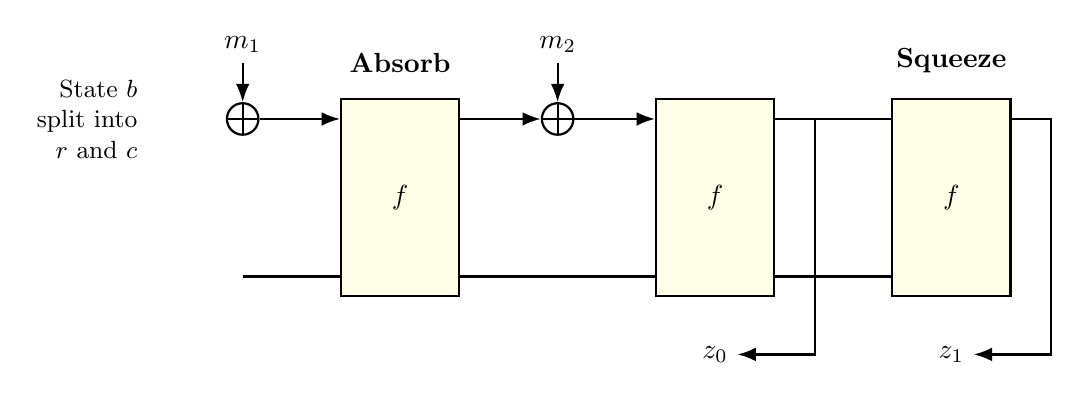
\begin{tikzpicture}[
        node distance=1.5cm,
        perm/.style={rectangle, draw=black, thick, fill=yellow!10, minimum width=1.5cm, minimum height=2.5cm, align=center},
        r_part/.style={rectangle, draw=blue!80!black, thick, fill=blue!5, minimum width=1.5cm, minimum height=1cm, label=center:$r$},
        c_part/.style={rectangle, draw=red!80!black, thick, fill=red!5, minimum width=1.5cm, minimum height=1.5cm, label=center:$c$},
    ]
        % --- ABSORB PHASE ---
        \node[xor] (X1) at (0, 2) {};
        \node[above=0.5cm of X1] (M1) {$m_1$};
        \draw[arrow] (M1) -- (X1);
        
        \node[perm] (F1) at (2, 1) {$f$};
        \draw[arrow] (X1) -- (F1.west |- X1);      % r goes in
        \draw[thick] (0, 0) -- (F1.west |- 0,0);   % c goes in (init 0)
        
        \node[xor] (X2) at (4, 2) {};
        \node[above=0.5cm of X2] (M2) {$m_2$};
        \draw[arrow] (M2) -- (X2);
        
        \draw[arrow] (F1.east |- X2) -- (X2);      % r out to next XOR
        \node[perm] (F2) at (6, 1) {$f$};
        \draw[arrow] (X2) -- (F2.west |- X2);      % r in
        \draw[thick] (F1.east |- 0,0) -- (F2.west |- 0,0); % c pass through
        
        % --- SQUEEZE PHASE ---
        \node[perm] (F3) at (9, 1) {$f$};
        \draw[thick] (F2.east |- 2,2) -- (F3.west |- 2,2);
        \draw[thick] (F2.east |- 0,0) -- (F3.west |- 0,0);
        
        % Outputs
        \node[below=0.5cm of F2] (Z0) {$z_0$};
        \draw[arrow] (F2.east |- 2,2) -- ++(0.5,0) |- (Z0);
        
        \node[below=0.5cm of F3] (Z1) {$z_1$};
        \draw[arrow] (F3.east |- 2,2) -- ++(0.5,0) |- (Z1);
        
        % Annotations
        \node[above=0.2cm of F1, font=\bfseries] {Absorb};
        \node[above=0.2cm of F3, font=\bfseries] {Squeeze};
        
        % Legend for state
        \node[left=1cm of X1, font=\small, align=right] {State $b$\\split into\\$r$ and $c$};

    \end{tikzpicture}
    \caption{The Sponge Construction. $r$ determines speed, $c$ determines security.}
\end{figure}

\subsection{Comparison}

\begin{table}[H]
    \centering
    \renewcommand{\arraystretch}{1.5}
    \begin{tabular}{@{} l p{6cm} p{6cm} @{}}
        \toprule
        \textbf{Feature} & \textbf{SHA-2 (Merkle-Damgård)} & \textbf{SHA-3 (Sponge)} \\
        \midrule
        \textbf{Structure} & Iterative Compression ($H_{i} = f(H_{i-1}, m_i)$) & Permutation-based state update \\
        \textbf{Operations} & Add (mod $2^{32}/2^{64}$), Rotate, XOR, Shift & XOR, AND, NOT, Rotate (No arithmetic add) \\
        \textbf{Vulnerabilities} & Susceptible to Length Extension Attacks (without HMAC) & Resistant to Length Extension Attacks \\
        \textbf{Flexibility} & Fixed output length per variant & Extendable Output Function (XOF) \\
        \bottomrule
    \end{tabular}
    \caption{Comparison of modern hash standards.}
\end{table}


\section{SSL/TLS Protocol}

\subsection{Formal Definition}
The TLS protocol (successor to SSL) provides privacy and data integrity between two communicating applications. It is composed of two layers:
\begin{enumerate}
    \item \textbf{The TLS Record Protocol:} Layered on top of a reliable transport (TCP), it ensures that the connection is private (using symmetric encryption) and reliable (using message authentication).
    \item \textbf{The TLS Handshake Protocol:} Allows the client and server to authenticate each other and negotiate encryption algorithms and cryptographic keys before the application protocol transmits or receives its first byte of data.
\end{enumerate}

\subsection{The TLS Handshake Protocol}
The handshake is the most complex part of TLS. Its goal is to establish a \textbf{Master Secret} from which session keys are derived.

\subsection{Protocol Flow (TLS 1.2 Full Handshake)}
We visualize the exchange involving a Diffie-Hellman Key Exchange (DHE) for Forward Secrecy.

\begin{figure}[H]
  \tikzset{
    packet/.style={rectangle, draw=blue!80!black, thick, fill=blue!5, align=center, minimum width=4.5cm, minimum height=0.8cm, rounded corners, font=\small},
    actor/.style={circle, draw=black, thick, minimum size=1.2cm, fill=gray!10, font=\bfseries},
    arrow/.style={-Latex, thick},
    line/.style={draw, thick},
    note/.style={font=\footnotesize, color=gray!80!black, align=left},
    encrypt/.style={rectangle, draw=red!80!black, thick, fill=red!5, align=center, minimum width=2.5cm},
    header/.style={rectangle, draw=black, thick, fill=yellow!10, minimum width=1cm}
}
    \centering
    \begin{tikzpicture}[node distance=0.6cm]
        % Actors
        \node[actor] (Client) {Client};
        \node[actor, right=8cm of Client] (Server) {Server};
        
        % 1. Client Hello
        % Position: centered between client/server, dropped down
        \node[packet, below=1.5cm of Client, anchor=west, xshift=1.75cm] (CH) {\textbf{ClientHello}\\$R_C$, CipherSuites, Ver};
        \draw[arrow] (Client |- CH) -- (Server |- CH);

        % 2. Server Hello
        \node[packet, below=of CH] (SH) {\textbf{ServerHello}\\$R_S$, Selected Cipher, Ver};
        \draw[arrow] (Server |- SH) -- (Client |- SH);

        % 3. Certificate
        \node[packet, below=of SH] (Cert) {\textbf{Certificate}\\$pk_{server}$};
        \draw[arrow] (Server |- Cert) -- (Client |- Cert);

        % 4. Server Key Exchange
        \node[packet, below=of Cert] (SKE) {\textbf{ServerKeyExchange}\\params: $g, p, g^b$, Sig};
        \draw[arrow] (Server |- SKE) -- (Client |- SKE);

        % 5. Server Hello Done
        \node[packet, below=of SKE, fill=white, draw=black] (SHD) {ServerHelloDone};
        \draw[arrow] (Server |- SHD) -- (Client |- SHD);

        % Client Processing Note
        \node[note, left=0.5cm of SHD, align=right] (Proc) {
            \textbf{Processing:}\\
            Verify Cert \& Sig\\
            Gen Secret $a$\\
            Calc PMS ($g^{ab}$)
        };

        % 6. Client Key Exchange
        \node[packet, below=1.5cm of SHD] (CKE) {\textbf{ClientKeyExchange}\\$g^a$};
        \draw[arrow] (Client |- CKE) -- (Server |- CKE);

        % 7. Change Cipher Spec
        \node[packet, below=of CKE, fill=yellow!10] (CCS) {\textbf{ChangeCipherSpec}};
        \draw[arrow] (Client |- CCS) -- (Server |- CCS);

        % 8. Finished
        \node[packet, below=of CCS, fill=red!10] (FinC) {\textbf{Finished}\\Enc(Hash(Msgs))};
        \draw[arrow] (Client |- FinC) -- (Server |- FinC);

        % 9. Server Change Cipher Spec
        \node[packet, below=of FinC, fill=yellow!10] (SCCS) {\textbf{ChangeCipherSpec}};
        \draw[arrow] (Server |- SCCS) -- (Client |- SCCS);

        % 10. Server Finished
        \node[packet, below=of SCCS, fill=red!10] (FinS) {\textbf{Finished}\\Enc(Hash(Msgs))};
        \draw[arrow] (Server |- FinS) -- (Client |- FinS);

        % Timelines
        % We draw these last so they go "behind" the filled packet nodes if layer order matters, 
        % but since nodes are opaque, drawing them first is usually safer. 
        % However, we needed the node positions to draw the arrows.
        % Let's draw the lines from Actor to the bottom.
        \coordinate (Bottom) at ($(FinS)+(0,-1.5)$);
        \draw[thick] (Client) -- (Client |- Bottom);
        \draw[thick] (Server) -- (Server |- Bottom);

        % Secure Channel Indicator
        \draw[line width=2pt, green!50!black, <->] ($(Client |- Bottom) + (0,0.5)$) -- node[above, fill=white, font=\bfseries] {Secure Channel Established} ($(Server |- Bottom) + (0,0.5)$);

    \end{tikzpicture}
    \caption{TLS 1.2 Full Handshake with Diffie-Hellman Key Exchange.}
\end{figure}

\subsection{Key Derivation}
The security of TLS relies on deriving symmetric keys from the material exchanged in the handshake.

\subsection{The Pre-Master Secret (PMS)}
Depending on the key exchange method:
\begin{itemize}
    \item \textbf{RSA:} Client generates a 48-byte random string and encrypts it with Server's public key.
    \item \textbf{Diffie-Hellman:} Both sides compute $g^{ab} \pmod p$.
\end{itemize}

\subsubsection{The Master Secret (MS)}
The MS is a 48-byte value calculated using a Pseudorandom Function (PRF):
\[
MS = \mathsf{PRF}(PMS, \text{"master secret"}, R_C + R_S)
\]
Where $R_C$ and $R_S$ are the client and server random nonces sent in the Hello messages.

\subsubsection{Session Keys}
The Master Secret is expanded to generate the \textbf{Key Block}, which is sliced into:
\begin{itemize}
    \item Client Write MAC Key
    \item Server Write MAC Key
    \item Client Write Encryption Key
    \item Server Write Encryption Key
    \item (IVs for block ciphers)
\end{itemize}

\subsection{The TLS Record Protocol}
Once the handshake is complete, the Record Protocol takes application data and secures it.

\begin{figure}[H]
  \tikzset{
    packet/.style={rectangle, draw=blue!80!black, thick, fill=blue!5, align=center, minimum width=4.5cm, minimum height=0.8cm, rounded corners, font=\small},
    actor/.style={circle, draw=black, thick, minimum size=1.2cm, fill=gray!10, font=\bfseries},
    arrow/.style={-Latex, thick},
    line/.style={draw, thick},
    note/.style={font=\footnotesize, color=gray!80!black, align=left},
    encrypt/.style={rectangle, draw=red!80!black, thick, fill=red!5, align=center, minimum width=2.5cm},
    header/.style={rectangle, draw=black, thick, fill=yellow!10, minimum width=1cm}
}
    \centering
    \begin{tikzpicture}[node distance=1cm]
        % Styles
        \tikzstyle{proc}=[rectangle, draw=black, thick, fill=white, align=center, minimum height=1cm];
        
        % Input
        \node[packet, fill=gray!10] (Data) {Application Data stream};
        
        % Frag
        \node[proc, below=0.8cm of Data] (Frag) {Fragmentation\\($\le 2^{14}$ bytes)};
        
        % Compress
        \node[proc, below=0.8cm of Frag] (Comp) {Compression\\(Optional/Null)};
        
        % MAC
        \node[proc, below=0.8cm of Comp] (MAC) {Compute MAC\\$HMAC(K_{mac}, \text{seq} + \text{header} + \text{data})$};
        
        % Encrypt
        \node[proc, below=0.8cm of MAC, fill=red!5, draw=red!80!black] (Enc) {Encryption\\$E(K_{enc}, \text{data} + \text{MAC} + \text{Pad})$};
        
        % Header
        \node[proc, below=0.8cm of Enc, fill=yellow!10] (Header) {Prepend Header\\(Type, Ver, Len)};
        
        % Output
        \node[packet, below=0.8cm of Header, fill=green!10] (TLS) {TLS Record};
        
        % Arrows
        \draw[arrow] (Data) -- (Frag);
        \draw[arrow] (Frag) -- (Comp);
        \draw[arrow] (Comp) -- (MAC);
        \draw[arrow] (MAC) -- (Enc);
        \draw[arrow] (Enc) -- (Header);
        \draw[arrow] (Header) -- (TLS);
        
        % Structure visual
        \node[right=1.5cm of TLS] (Struct) {
            \begin{tikzpicture}
                \node[header] (H) {Hdr};
                \node[encrypt, right=0cm of H] (Pay) {Encrypted Data + MAC};
            \end{tikzpicture}
        };
        \draw[dashed, ->] (TLS) -- (Struct);

    \end{tikzpicture}
    \caption{The TLS Record Protocol Processing Stack.}
\end{figure}

\subsection{Security Services Provided}
\begin{itemize}
    \item \textbf{Confidentiality:} Achieved via symmetric encryption (AES, ChaCha20) using keys derived from the Master Secret.
    \item \textbf{Integrity:} Achieved via HMAC or AEAD (Authenticated Encryption with Associated Data).
    \item \textbf{Authentication:} Achieved via Certificates (X.509) and Digital Signatures (RSA/ECDSA) during the handshake.
    \item \textbf{Replay Protection:} Implicitly provided by the sequence numbers used in the MAC calculation.
\end{itemize}

\end{document}